\documentclass[12pt]{article}

% All figures and generated tables live in presentation_assets/ to keep Overleaf portability.

\usepackage[]{graphicx}
\graphicspath{{presentation_assets/fig/}}
\usepackage[]{color}
\usepackage{alltt}
\usepackage{amsmath}
\usepackage{amssymb}
\usepackage{multirow}
\usepackage{booktabs}
\usepackage{placeins}

\newcommand{\mytitle}{Variance-Based Analysis of Predictive Multiplicity in Rashomon Sets}
\newcommand{\myname}{Dejvis Toptani}
\newcommand{\mysupervisor}{Dr. Giuseppe Casalicchio}

\usepackage[a4paper, width = 160mm, top = 35mm, bottom = 30mm, 
bindingoffset = 0mm]{geometry}
\usepackage[utf8]{inputenc}
\usepackage{ragged2e}
\usepackage{xcolor}
\usepackage[round, comma]{natbib}
\usepackage{fancyhdr}
\newcommand{\changefont}{%
    \fontsize{8}{11}\selectfont
}
\usepackage{hyperref}
\hypersetup{
  colorlinks = true,
  linkcolor = black,
  urlcolor = black,
  citecolor = black}
\pagestyle{fancy}
\fancyhead{}
\fancyhead[R]{\changefont{\mytitle}}
\fancyfoot{}
\fancyfoot[R]{\thepage}
\setlength{\headheight}{14.5pt}
\setlength{\parindent}{0pt}
\interfootnotelinepenalty = 10000

% ------------------------------------------------------------------------------
% MAIN -------------------------------------------------------------------------
% ------------------------------------------------------------------------------
\IfFileExists{upquote.sty}{\usepackage{upquote}}{}
\begin{document}

% FRONT PAGE -------------------------------------------------------------------
 
\begin{titlepage}
\begin{center}
    
\LARGE
Master's Thesis
    
\vspace{0.5cm}
      
\rule{\textwidth}{1.5pt}
\LARGE
\textbf{\mytitle}
\rule{\textwidth}{1.5pt}
   
\vspace{0.5cm}
      
\large
Department of Statistics \\
Ludwig-Maximilians-Universität München 

\vfill

\Large
\textbf{\myname}

\vfill

\large
Munich, June 29\textsuperscript{th}, 2026
      
\vfill

% TODO: missing figure file sigillum.png -- add it to presentation_assets/fig/

\includegraphics[width = 0.4\textwidth]{sigillum.png}

\vfill

\normalsize
Submitted in partial fulfillment of the requirements for the degree of M. Sc.
\\

Supervised by \mysupervisor

\end{center}
\end{titlepage}

% CONTENTS ---------------------------------------------------------------------

\pagenumbering{Roman}
\newpage

\begin{abstract}

Modern machine learning pipelines often produce many models with near-identical predictive performance, yet these models can disagree substantially on individual predictions—a phenomenon known as \emph{predictive multiplicity}. Existing approaches quantify this disagreement at the aggregate level but do not reveal \emph{where} in the feature space it concentrates or \emph{which} modeling choices drive it.

This thesis introduces a spatial analysis framework for predictive multiplicity. We compute observation-wise predictive variance across a Rashomon set of near-optimal models and analyze its structure using spatial statistics, including global Moran’s $I$ and Local Indicators of Spatial Association (LISA). This enables the detection, localization, and statistical validation of \emph{multiplicity hotspots}—regions in feature space where predictions are particularly model-dependent. We further decompose predictive variance into between-family and within-family (hyperparameter) components and analyze how these drivers vary across the feature space.

Experiments on three benchmark datasets with five model families confirm that predictive multiplicity is consistently spatially structured and non-random. Model family accounts for a substantial share of disagreement, with particularly strong
hotspot-specific contributions on COMPAS and Adult. These patterns are robust to changes in Rashomon set size, neighborhood definition, probability calibration, and graph construction. Synthetic experiments with known ambiguous regions validate the pipeline's ability to recover ground-truth instability. High-multiplicity regions can additionally be characterized by compact, interpretable rules in the original feature space.

The results suggest that predictive multiplicity is not merely a global property of model classes, but a localized phenomenon affecting specific subpopulations. The proposed framework provides a practical diagnostic for identifying predictions that are especially sensitive to model choice, with implications for the reliability, fairness, and governance of automated decision systems.

\end{abstract}

\newpage
\tableofcontents

%%%% if you would want to include material overview
%%%% use one of the following in addition
% \newpage
% \listoffigures
% \newpage
% \listoftables
\newpage

% CHAPTERS ---------------------------------------------------------------------

\pagenumbering{arabic}
    
\section{Introduction}
\label{intro}
Supervised machine learning (ML) models are increasingly used to support decisions in domains such as healthcare, finance, and criminal justice. Their appeal lies in strong predictive performance, but high performance alone does not guarantee reliable or trustworthy predictions. In modern ML pipelines, many distinct models often achieve nearly identical predictive accuracy on the same task, yet still differ substantially in their predictions for individual observations. Classical evaluation metrics such as accuracy, AUC, or Brier score summarize average model quality, but they provide little insight into whether a specific prediction is stable or whether it depends strongly on which near-optimal model happens to be selected.

This phenomenon is known as \emph{predictive multiplicity}: multiple models that are essentially indistinguishable in overall performance can still disagree in meaningful ways at the level of individual decisions. This creates an important reliability problem for automated decision systems. If several equally accurate models exist, then a prediction may reflect not only the data, but also an arbitrary modeling choice within a broader set of acceptable alternatives. In high-stakes settings, this raises a natural question: are all predictions from a well-performing model equally trustworthy, or are some individuals especially exposed to model-dependent instability?

In this thesis, we study predictive multiplicity through a spatial lens. Rather than asking only \emph{how much} near-optimal models disagree on average, we ask whether this disagreement is concentrated in specific regions of the feature space, whether these regions are stable, and which modeling choices drive them. To answer these questions, we propose a framework that combines observation-wise predictive variance with tools from spatial statistics to detect, localize, and interpret regions of concentrated instability.

\subsection{Motivation}

Automated decision systems are often deployed as if the selected model were the unique and definitive representation of the relationship between inputs and outcomes. In practice, however, this assumption is rarely justified. Modern training pipelines typically generate many models that perform almost equally well, especially when multiple model families, hyperparameter settings, and random initializations are considered. From a global performance perspective, these models may all appear equally valid. From an individual perspective, however, they may produce substantially different predictions.

This matters because many consequential decisions are made at the individual level. A credit application is approved or rejected for a particular person; a patient is assigned a risk score; a defendant is classified as high or low risk. If such decisions depend strongly on which near-optimal model is selected, then average predictive performance alone is not an adequate description of system reliability. The following fictional examples illustrate the central ideas of this thesis.

\subsubsection{Example 1: Prediction Instability at the Individual Level}

Alice is evaluated by an automated risk assessment system. The deployed model predicts a probability of 0.29 that she will reoffend within two years, classifying her as ``low risk.'' During an audit, however, the analyst examines not only the deployed model, but all models whose validation performance lies within a small tolerance of the optimum. Although these models are essentially indistinguishable in overall accuracy, their predictions for Alice range from 0.22 to 0.54.

The variance of Alice's predicted risk across these equally accurate models is high, placing her among the most unstable individuals in the dataset. Whether Alice is classified as low risk or high risk therefore depends not only on the observed data, but also on which near-optimal model happened to be chosen. Her case illustrates the core problem of predictive multiplicity: a system can appear stable at the aggregate level while remaining unstable for specific individuals.

\subsubsection{Example 2: Spatial Clustering of Instability}

An auditor then asks whether cases like Alice are isolated exceptions or part of a broader pattern. By mapping prediction-instability scores across the feature space, the auditor finds that high-instability observations are not randomly scattered. Instead, they cluster in specific regions. A spatial autocorrelation test confirms that this concentration is unlikely to be due to chance.

These clusters correspond to subpopulations for whom predictions are systematically more model-dependent than for others. In such regions, the choice among equally accurate models has an especially large effect on the final output. This shifts the interpretation of reliability: the question is no longer only whether a model performs well overall, but also where in the population its predictions are most contingent on arbitrary model selection.

\subsubsection{Example 3: Drivers of Instability}

The next question is why such instability occurs. The auditor decomposes the observed predictive variance and finds that some of it is explained by broad modeling choices, such as whether the system uses logistic regression, tree-based models, or neural networks. Additional variation arises within families from hyperparameter choices such as regularization strength, tree depth, or learning rate. Moreover, these drivers are not spatially uniform: some modeling choices matter much more inside instability hotspots than outside them.

\medskip

Together, these examples illustrate the main thesis perspective: predictive multiplicity is not merely a global nuisance, but can be a spatially structured phenomenon that concentrates in identifiable regions, affects specific subpopulations, and is shaped by identifiable modeling choices. Understanding \emph{where} such instability occurs and \emph{what drives it} is essential for developing more reliable and transparent automated decision systems.

\subsection{Predictive Multiplicity and Rashomon Sets}

The phenomenon described above is closely related to two established ideas in the literature. \emph{Predictive multiplicity} \citep{marx_predictive_2020} refers to the situation in which models with similar predictive performance nonetheless produce conflicting predictions for individual observations. The broader \emph{Rashomon effect} \citep{breiman_statistical_2001} captures the idea that many distinct models may explain the same data almost equally well.

The collection of near-optimal models is called the \emph{Rashomon set}:
\[
\mathcal{R}_\varepsilon = \{ f \in \mathcal{F} : L(f) \leq L^* + \varepsilon \},
\]
where $L^*$ denotes the best achievable loss within the candidate class and $\varepsilon$ specifies the allowed performance tolerance. Prior work has studied predictive multiplicity using quantities such as ambiguity, discrepancy, and disagreement rate. These measures capture important aspects of disagreement, but they are primarily global summaries. They describe how much near-optimal models differ on average, yet they do not reveal whether disagreement is concentrated in specific local regions of the feature space.

\subsection{Problem Statement}

Predictive models with nearly identical overall performance can differ substantially in their predictions. Such variation arises naturally in realistic ML pipelines through differences in model family, hyperparameter choices, optimization paths, or random seeds. Existing multiplicity metrics mainly quantify disagreement at the aggregate level. They do not reveal whether disagreement is spatially concentrated, which kinds of observations form high-multiplicity regions, or how to distinguish between the influence of model family and within-family hyperparameters.

As a result, users of automated decision systems lack a principled way to identify which predictions are robust across acceptable models and which are highly contingent on arbitrary modeling choices. The problem addressed in this thesis is therefore to characterize and quantify predictive multiplicity at the observation level, with particular emphasis on its \emph{spatial structure} in feature space and its \emph{drivers} across model classes and hyperparameters.

\subsection{Research Questions}

Building on this problem statement, this thesis investigates the following research questions:

\begin{enumerate}
    \item \textbf{Prediction-Level Multiplicity.}  
    How much do individual predictions vary across equally accurate models, which observations are most affected, and does this variation exceed what would be expected under a chance baseline?

    \item \textbf{Spatial Structure of Multiplicity.}  
    Does observation-wise predictive variance exhibit spatial autocorrelation in feature space? Can we identify contiguous hotspot regions---localized clusters of elevated disagreement---in which near-optimal models systematically diverge?

    \item \textbf{Stability of Spatial Patterns.}  
    Are the identified hotspot regions stable across different train/validation/test splits and Rashomon set realizations, or are they primarily artifacts of random variation?

    \item \textbf{Drivers of Multiplicity.}  
    How much of the predictive variance is explained by model family versus hyperparameters within each family, and do these drivers differ between hotspot and non-hotspot regions?

    \item \textbf{Robustness and Sensitivity.}  
    Are the spatial multiplicity findings robust to the Rashomon set size $K$, the neighborhood size $k$ used in the feature-space graph, and post-hoc probability calibration?

    \item \textbf{Validation.}  
    Does the proposed pipeline recover known ambiguous regions when applied to synthetic data with ground-truth instability?

    \item \textbf{Interpretable Characterization.}  
    Can high-multiplicity regions be described by simple, interpretable rules in terms of the original feature space?
\end{enumerate}

\subsection{Contributions of This Thesis}

This thesis makes four main contributions.

\begin{enumerate}
    \item \textbf{A spatial framework for predictive multiplicity.}  
    We propose a pipeline that combines observation-wise predictive variance with spatial autocorrelation methods to detect, localize, and test for significant clusters of disagreement in feature space.

    \item \textbf{Empirical evidence across datasets and seeds.}  
    We evaluate the framework on three benchmark datasets with multiple outer runs, five model families, and large candidate pools, showing that predictive multiplicity often exhibits clear spatial structure rather than appearing as diffuse noise.

    \item \textbf{Attribution of disagreement to modeling choices.}  
    We decompose predictive variance into between-family and within-family components, identifying which model classes and hyperparameters drive instability globally and within localized hotspot regions.

    \item \textbf{Robustness and interpretability analyses.}  
    We show that the main spatial findings are robust to several analytical choices, validate the pipeline on synthetic data with known ambiguous regions, and extract compact decision rules that characterize the affected subpopulations.
\end{enumerate}

\subsection{Thesis Structure}

The remainder of this thesis is organized as follows. Chapter~2 reviews related work on predictive multiplicity, Rashomon sets, model disagreement, and spatial localization. Chapter~3 presents the methodological framework, including Rashomon-set construction, observation-wise multiplicity metrics, feature-space graphs, spatial statistics, and null testing. Chapter~4 describes the experimental design, including datasets, preprocessing, model families, Rashomon operationalization, and robustness analyses. Chapter~5 presents the empirical results. Chapter~6 discusses the findings, implications, and limitations. Chapter~7 concludes and outlines directions for future work.
\newpage

\section{Background and Related Work}
\label{related}
% ===================================================================
% Background and Related Work — revised to focus on literature that
% directly motivates the thesis contribution.
% ===================================================================

Predictive multiplicity lies at the intersection of three lines of work: the study of
Rashomon sets, the design of metrics that quantify disagreement among near-optimal
models, and the broader question of what such disagreement implies for model selection,
fairness, and reliability. The central observation is that a single deployed model is often
only one choice among several similarly well-performing alternatives. Even when a
machine-learning workflow ultimately returns one final model, other choices of model
family, hyperparameters, or random seed may lead to models with nearly identical
predictive performance but different outputs for the same individual. This chapter
reviews the literature most directly connected to that observation and uses it to motivate
the perspective taken in this thesis: predictive multiplicity should be studied not only as
a global property of a dataset or model class, but also as a localized phenomenon in
feature space.

% -------------------------------------------------------------------
\subsection{Rashomon Sets and Predictive Multiplicity}
% -------------------------------------------------------------------

The modern formulation of multiplicity is rooted in the \emph{Rashomon effect},
introduced by \cite{breiman_statistical_2001}. The Rashomon effect describes the situation in which many distinct models achieve
similarly good predictive performance, while relying on different functional forms,
variables, or relationships in the data. In other words, there may be no single
uniquely best explanation of the data-generating relationship. This perspective is also
used by \cite{fisher2019all}, who argue that conclusions drawn from one fitted model
can be incomplete when other well-performing models rely on different variables or
relationships.

Formally, let $\mathcal{F}$ be a hypothesis class, let $L(f)$ be the loss of a model
$f \in \mathcal{F}$, and let $L^* = \min_{f \in \mathcal{F}} L(f)$ be the best loss in this
class. The corresponding \emph{Rashomon set} is
\[
  \mathcal{R}_\varepsilon
  = \bigl\{f \in \mathcal{F} : L(f) \leq L^{*} + \varepsilon\bigr\}.
\]
It contains all models whose loss is within a tolerance $\varepsilon$ of the best model.
This shifts attention from a single selected model to a set of near-optimal alternatives.

Recent Rashomon-set research has emphasized that the size and structure of
$\mathcal{R}_\varepsilon$ can have substantial practical consequences.
\cite{semenova_existence_2022} formalize the \emph{Rashomon ratio}, i.e., the volume of
$\mathcal{R}_\varepsilon$ relative to the hypothesis space, and argue that large Rashomon
sets help explain why simpler yet accurate models may exist.
\cite{rudin_amazing_2024} broaden this perspective further: when many good models are
available, model development should not be viewed as a search for a uniquely correct
solution, but as a search over a set of viable models that may differ in interpretability,
fairness, robustness, and other secondary properties.

Within this broader setting, \cite{marx_predictive_2020} introduce
\emph{predictive multiplicity} as the phenomenon that near-optimal models can assign
conflicting predictions to the same observation.
\cite{black_model_2022} generalize this concern under the broader notion of
\emph{model multiplicity}, highlighting that arbitrariness in model choice can create
both opportunities and risks: multiplicity may enable deliberate optimization for fairness
or interpretability, but it may also make individual outcomes depend on choices that are
invisible to affected stakeholders.

Predictive multiplicity should also be distinguished from classical notions of
uncertainty. Aleatoric uncertainty reflects inherent noise in the data, while epistemic
uncertainty captures limited knowledge about the data-generating process. In contrast,
predictive multiplicity arises from the existence of multiple equally accurate models
that produce different predictions for the same observation. The resulting disagreement
is therefore not due only to noise or lack of information, but to the structure of the
model space itself.

This thesis studies precisely that predictive facet of multiplicity: how much near-optimal
models disagree on individual observations, where that disagreement is concentrated, and
which modeling choices drive it.

% -------------------------------------------------------------------
\subsection{Metrics for Predictive Multiplicity}
\label{sec:metrics-review}
% -------------------------------------------------------------------

The first generation of predictive-multiplicity metrics operates in \emph{label space}.
\cite{marx_predictive_2020} propose \emph{ambiguity}, which measures how often a sample
can receive conflicting labels within the Rashomon set, and \emph{discrepancy}, which
quantifies the maximal extent of such disagreement. These measures made predictive multiplicity operational, but they reduce model outputs to binary decisions based on a fixed threshold (e.g., 0.5), thereby ignoring differences in predicted probabilities when models agree on the final label.

A second line of work extends multiplicity to \emph{probability space}.
\cite{watson-daniels_predictive_2023} develop a framework for predictive multiplicity in
probabilistic classification, introducing score-based measures that capture the variation
of risk estimates across near-optimal models rather than only label flips. Their analysis
also connects multiplicity to dataset characteristics such as separability, outliers, and
majority--minority structure. This is especially relevant for this thesis because the
main response variable is not hard disagreement alone, but the full spread of predicted
probabilities across the Rashomon set.

Closely related, \cite{hsu_rashomon_nodate} propose \emph{Rashomon Capacity}, an
information-theoretic measure of predictive multiplicity in probabilistic classification.
The measure is defined at the level of an individual observation and captures how much
the possible predicted scores for that observation vary across models in the Rashomon set.
\cite{hsu_rashomongb_2024} extend this line in the context of gradient boosting,
introducing \emph{RashomonGB} as a practical method for inspecting multiplicity in boosted
models and discussing score-based notions such as the \emph{Viable Prediction Range} for
individual observations.

At the per-observation level, one particularly useful hard-disagreement measure is the
\emph{conflict ratio}, which records the fraction of models on the minority side of a
decision threshold. Recent work by \cite{frohnapfel_using_2026} argues that such
individual-level multiplicity measures are not only methodologically useful but also
policy-relevant, because they can help operationalize per-person performance reporting
requirements in high-stakes settings under the EU AI Act.

Taken together, the literature now offers several ways to quantify multiplicity globally
and per instance, in both label space and probability space. What remains much less
developed is how to move from pointwise disagreement scores to an analysis of whether
disagreement forms coherent \emph{regions} in feature space.


\subsection{Localizing Instability in Feature Space}
\label{sec:spatial-review}
% -------------------------------------------------------------------

The metrics discussed above quantify predictive multiplicity either at the dataset level
or for individual observations. A remaining question is whether observations with high
prediction disagreement are isolated cases, or whether they form coherent regions in
feature space. This thesis approaches that question using tools from spatial statistics.

\cite{moran1950notes} introduced Moran's $I$ as a measure of global spatial
autocorrelation. In this thesis, it is used to test whether observations with similar
levels of prediction instability tend to be close to each other in feature space.
\cite{anselin1995local} developed \emph{Local Indicators of Spatial Association} (LISA),
which identify where such local clustering occurs. In particular, LISA can identify
\emph{High--High} regions, where observations with high values are surrounded by
neighbors that also have high values, and \emph{Low--Low} regions, where low values
cluster together.

In their original setting, these tools operate on geographic data with an explicit spatial
adjacency structure. In this thesis, the same logic is transferred to
\emph{feature space}: observations become nodes in a $k$-nearest-neighbor graph, and
observation-wise multiplicity scores become the variable whose spatial organization is
tested. Conceptually, this turns predictive multiplicity from a collection of isolated
pointwise values into a structured signal that can be analyzed for clustering, significance,
and local hotspot formation.

This step is motivated by observations already present in the literature on predictive
multiplicity. \cite{watson-daniels_predictive_2023} show that prediction disagreement
across near-optimal probabilistic classifiers is associated with dataset characteristics such
as outliers and separability. This suggests that predictive multiplicity may not be
distributed uniformly across the input space. Likewise, per-instance feasible-range
methods such as those discussed by \cite{hsu_rashomongb_2024} show that the range of
possible predictions can vary substantially from one observation to another. These works
therefore motivate an observation-level view of predictive multiplicity. However, they do
not directly analyze whether observations with high disagreement form statistically
significant, spatially contiguous regions in feature space.

That question matters for interpretation. Once disagreement is shown to cluster, the
relevant object is no longer only an unstable individual prediction, but an unstable
\emph{subpopulation}. This shifts the focus from isolated observations to coherent
regions of the feature space, enabling a more structured analysis of where and how
predictive multiplicity arises.


% -------------------------------------------------------------------
\subsection{Drivers and Consequences of Predictive Multiplicity}
\label{sec:drivers-review}
% -------------------------------------------------------------------

After asking how predictive multiplicity can be measured and localized, a further question
is why it arises and why it matters. One source is model selection itself. If several models
perform similarly well, then choosing one final model is not only a technical step, but can
affect individual predictions. \cite{black_model_2022} and \cite{rudin_amazing_2024}
emphasize this point: when many good models are available, model choice should be seen
as a substantive design decision, because different acceptable models may differ in other
properties such as interpretability, fairness, or robustness.

More recently, attention has turned to concrete modeling choices that generate
multiplicity within a model family. Most directly relevant for this thesis is
\cite{cavus_role_2025}, who show across benchmark datasets that hyperparameter tuning
can materially increase prediction discrepancy even when performance improves.
Their results suggest that multiplicity is not driven only by broad differences between
families such as linear models versus tree ensembles, but also by movement through
hyperparameter space within a fixed family.

Recent work also highlights that prediction variance across models can lead to
arbitrary decisions for individual observations \citep{cooper2024arbitrariness}.

The implications of such disagreement have also been studied from a fairness and
governance perspective. \cite{sokol_cross-model_2024} formulate
\emph{cross-model fairness}, emphasizing that when different equally performing models
treat the same person differently, fairness concerns arise not only from the deployed
predictor itself but also from the unresolved choice among competing predictors.
Similarly, \cite{frohnapfel_using_2026} connect predictive multiplicity to legal and
reporting obligations in high-risk decision support, arguing that disagreement across
near-optimal models can be interpreted as a form of person-level arbitrariness that should
be made visible to deployers.

These works clarify why multiplicity matters and which modeling choices may create it.
However, they mostly operate at the level of whole datasets, whole model classes, or
individual cases taken one at a time. They do not yet ask whether family effects and
hyperparameter effects become especially strong in \emph{specific parts} of feature space.


% -------------------------------------------------------------------
\subsection{Positioning of This Thesis}
% -------------------------------------------------------------------

The existing literature provides concepts and metrics for studying predictive
multiplicity, but it mostly treats disagreement either as a dataset-level quantity or as a
property of individual observations. Less attention has been given to whether these
observation-level differences form coherent regions in feature space.

This thesis addresses this gap by treating prediction instability as a spatial signal. It uses
observation-wise predictive variance to identify where near-optimal models disagree, and
then analyzes whether high-disagreement observations cluster locally. The goal is therefore not only to measure how much predictive
multiplicity exists, but also to locate where it occurs, assess how stable these regions
are, and examine which modeling choices are associated with them.

In this way, the thesis connects predictive multiplicity with a regional view of model
reliability: some parts of the feature space may be more sensitive to model choice than
others, even when all considered models perform similarly well overall.
\newpage

\section{Methodology}
\label{methodology}

This chapter presents the methodology used to analyze predictive multiplicity through a spatial lens. The proposed approach characterizes how predictions vary across a set of near-optimal models and investigates whether this variation exhibits statistically significant structure in feature space. The methodology is independent of any particular dataset or experimental configuration; dataset-specific choices are described in Chapter~4.

\subsection{Problem Setting and Notation}

Let $(X, y)$ denote a supervised learning dataset with $N$ observations, where $X \in \mathbb{R}^{N \times d}$ is the feature matrix and $y \in \{0,1\}^N$ is a binary target variable. Let $\mathcal{F}$ denote a hypothesis class of predictive models, potentially spanning multiple model families and hyperparameter configurations.

We consider probabilistic classifiers $f \in \mathcal{F}$ that output predicted probabilities $\hat{p}_{fi} \in [0,1]$ for each observation $i \in \{1,\dots,N\}$. Model performance is measured using a loss function $L(f)$ evaluated on held-out data.

\subsection{Rashomon Set of Near-Optimal Models}

Predictive multiplicity is studied through the Rashomon set, defined as the collection of models whose performance lies within a tolerance $\varepsilon > 0$ of the best achievable loss. Formally, let
\[
L^* = \min_{f \in \mathcal{F}} L(f)
\]
denote the minimal loss over all trained models. The Rashomon set is then defined as
\[
\mathcal{R}_\varepsilon = \{ f \in \mathcal{F} : L(f) \leq L^* + \varepsilon \}.
\]

The tolerance parameter $\varepsilon$ controls the strictness of the selection: smaller values yield a more homogeneous set of models, while larger values admit greater diversity. In practice, the Rashomon set can be operationalized by selecting a fixed number $K$ of best-performing models (top-$K$ by validation loss) to ensure comparable set sizes across runs and datasets; sensitivity to $K$ is examined empirically.

\subsection{Observation-Wise Predictive Variance}

To quantify predictive multiplicity at the level of individual observations, we compute the variance of predicted probabilities across the Rashomon set. Let $|\mathcal{R}_\varepsilon| = M$ denote the number of models in the Rashomon set, and let $\hat{p}_{mi}$ denote the predicted probability for observation $i$ produced by model $m \in \mathcal{R}_\varepsilon$.

The observation-wise predictive variance is defined as
\[
v_i = \mathrm{Var}_{m \in \mathcal{R}_\varepsilon}(\hat{p}_{mi}), \quad i = 1,\dots,N.
\]

This yields a scalar instability score for each observation, capturing the magnitude of disagreement among near-optimal models. Unlike range-based or binary disagreement metrics, predictive variance reflects the full distribution of predictions within the Rashomon set.

\subsection{Feature-Space Graph Construction}

To study the spatial organization of predictive variance, we represent the dataset as a graph in feature space. Observations are treated as nodes, and edges encode local neighborhood relationships.

A $k$-nearest-neighbor (kNN) graph is constructed using the feature vectors in $X$. Each observation is connected to its $k$ nearest neighbors according to a chosen distance metric. The resulting adjacency structure is represented by a row-normalized spatial weight matrix $W \in \mathbb{R}^{N \times N}$, where $W_{ij} > 0$ indicates that observation $j$ is a neighbor of observation $i$.

This graph provides the spatial structure required for subsequent autocorrelation and clustering analyses.

\subsection{Global Spatial Autocorrelation}

To test whether predictive variance is spatially structured in feature space, we compute the global Moran's $I$ statistic. Let $\mathbf{v} = (v_1, \dots, v_N)^\top$ denote the vector of observation-wise predictive variances, and let $\bar{v}$ denote its mean.

Global Moran's $I$ is defined as
\[
I = \frac{\sum_{i=1}^N \sum_{j=1}^N W_{ij} (v_i - \bar{v})(v_j - \bar{v})}
{\sum_{i=1}^N (v_i - \bar{v})^2}.
\]

Positive values of $I$ indicate that observations with similar levels of predictive variance tend to be neighbors in feature space, while values near zero suggest spatial randomness.

Statistical significance is assessed using permutation tests: the variance values are randomly permuted across observations while the spatial structure encoded by $W$ is held fixed. For local Moran statistics, significance is assessed per observation via permutation, and the Benjamini--Hochberg procedure is applied to control the false discovery rate (FDR) when identifying significant hotspots.

\subsection{Local Indicators of Spatial Association}

While global Moran's $I$ assesses overall spatial dependence, it does not identify where such dependence occurs. To localize regions of elevated predictive multiplicity, we compute Local Indicators of Spatial Association (LISA).

For each observation $i$, the local Moran statistic is defined as
\[
I_i = (v_i - \bar{v}) \sum_{j=1}^N W_{ij} (v_j - \bar{v}).
\]

Permutation-based significance tests are performed independently for each observation. Based on the sign of $v_i - \bar{v}$ and the local spatial lag, observations are assigned to one of four categories: High--High (HH), Low--Low (LL), High--Low (HL), or Low--High (LH). Observations that do not reach statistical significance after FDR correction are labeled as non-significant.

High--High observations correspond to locally unstable regions in which high predictive variance is surrounded by similarly unstable neighbors.

\subsection{Connected Components of High-Multiplicity Regions}

To extract coherent regions of predictive multiplicity, we restrict the kNN graph to observations classified as High--High and identify connected components within this subgraph.

Each connected component represents a contiguous region of feature space in which predictive variance is consistently elevated. Components below a minimum size threshold may be discarded to avoid spurious detections. The resulting components support region-level analysis and stability assessments across different data splits or Rashomon set realizations.

\subsection{Null Models for Spatial Multiplicity}

To ensure that detected spatial structure is not an artifact of marginal variance distributions, we employ null models based on permutation of predictions.

Specifically, predictions are permuted independently within each model across observations, preserving the overall distribution of predictions for each model while destroying any alignment between predictive variance and feature space. Observation-wise variance and spatial statistics are recomputed on the permuted data.

Comparing observed statistics to their null distributions allows us to assess whether spatial clustering of predictive variance exceeds what would be expected under spatial randomness.

\subsection{Hyperparameter Variance Decomposition}

To investigate the sources of predictive multiplicity, we decompose observation-wise variance into contributions attributable to hyperparameter choices.

For a given hyperparameter $h$, models in the Rashomon set are grouped according to their value of $h$. For each observation, total variance is decomposed into between-group and within-group components:
\[
\mathrm{Var}_{\text{total}} = \mathrm{Var}_{\text{between}}(h) + \mathrm{Var}_{\text{within}}(h).
\]

This decomposition quantifies how much of the predictive instability for each observation is explained by differences in hyperparameter values versus residual variation within hyperparameter groups. Aggregating these quantities across observations provides a principled measure of hyperparameter importance for predictive multiplicity.

\subsection{Calibration Robustness Check}

To test whether detected spatial multiplicity is driven by probability miscalibration rather than genuine disagreement, we apply a post-hoc calibration step. Platt scaling (a logistic regression fitted on predicted probabilities versus true labels) is fit on the \emph{validation set only} and applied to test-set predictions for each model in the Rashomon set. Multiplicity and spatial metrics (mean variance, Moran's $I$, LISA HH masks) are then recomputed on the calibrated predictions. If spatial structure were largely an artifact of miscalibration, we would expect Moran's $I$ and HH regions to change substantially after calibration; persistence of structure indicates that multiplicity reflects genuine prediction disagreement.

\subsection{Validation on Synthetic Data}

To validate that LISA HH regions correspond to genuinely ambiguous regions in feature space, we evaluate on synthetic datasets with \emph{known} ground-truth ambiguous regions. These datasets combine well-separated stable regions (where models tend to agree) with designed ``islands'' where the conditional probability $P(y=1|x)$ is near 0.5, so that near-optimal models can disagree. Recovery of these ground-truth regions by the HH classification (e.g.\ precision, recall, Jaccard overlap) provides a quantitative validation criterion for the spatial multiplicity pipeline.

\subsection{Interpretable Rule Extraction}

Once high-multiplicity regions have been identified via LISA (HH hotspots) or thresholding (top quantile of pointwise variance), a natural question is whether these regions can be described by simple, interpretable rules in terms of the original features. We frame this as a supervised classification task: label each test observation as belonging to the high-multiplicity region or not, then fit interpretable models to recover the labeling.

Four complementary methods are employed:
\begin{enumerate}
\item \textbf{Shallow decision trees.} A depth-limited decision tree is fitted to the binary label (HH or HV vs.\ rest). Each leaf defines a conjunctive rule; rules are evaluated by \emph{purity} (fraction of positives in the rule region) and \emph{support} (number of observations matched).
\item \textbf{L1-regularized logistic regression.} A logistic regression with L1 penalty identifies features with nonzero coefficients that are associated with high-multiplicity membership. The coefficient magnitudes indicate feature importance.
\item \textbf{Beam search for conjunctive rules.} A greedy beam search constructs conjunctions of feature conditions that maximize \emph{lift} (purity divided by base rate), subject to a minimum support constraint.
\item \textbf{Cluster-describe.} DBSCAN clustering of the high-multiplicity points in feature space identifies spatial clusters, and a decision tree is fitted to each cluster to produce cluster-specific rules.
\end{enumerate}

Rules are evaluated using purity, support, lift, and out-of-bag (OOB) stability under bootstrap resampling. Permutation enrichment tests assess whether the observed purity exceeds what would be expected by chance.

\subsection{Decision Boundary Proximity Analysis}

To test whether high-multiplicity regions are simply those near the decision boundary, we compute the margin $m_i = |\bar{p}_i - 0.5|$ for each test observation, where $\bar{p}_i$ is the ensemble mean predicted probability. We then compute the Pearson and Spearman correlations between pointwise variance and margin, and compare mean margins for HH vs.\ non-HH points using the Mann--Whitney U test.

\subsection{Fairness and Subgroup Exposure}

To assess whether HH and HV regions disproportionately affect demographic subgroups, we compute group-wise exposure rates: the fraction of each group's test points classified as HH (or HV), with uncertainty summarized by bootstrap confidence intervals across runs. For inferential reporting, we apply two safeguards: (i) per-run subgroup minimum size filtering, and (ii) minimum cross-run support for each subgroup. Significance is then evaluated with a \emph{stratified} permutation test: labels are shuffled within each run (preserving each run's sample composition), run-level rates are recomputed, and the aggregated inter-group disparity (max--min HH rate across eligible groups) is compared to its null distribution.

\subsection{Alternative Graph Constructions}

To verify that spatial results are not artifacts of the Euclidean distance metric on the full one-hot-encoded feature space, we compare the baseline kNN graph with two alternatives: (1) kNN in PCA-reduced space (retaining 15 components), and (2) kNN using cosine distance on L2-normalized features. All other pipeline parameters remain fixed; Moran's $I$ and HH counts are compared across methods.

\subsection{Summary}

The methodology described in this chapter provides a unified framework for analyzing predictive multiplicity as a spatial phenomenon. By combining Rashomon set analysis, observation-wise predictive variance, spatial statistics, null models, hyperparameter decomposition, calibration checks, validation on synthetic data, interpretable rule extraction, decision boundary proximity analysis, fairness exposure assessment, and alternative graph constructions, the approach enables identification, localization, interpretation, and description of regions in feature space where model predictions are particularly unstable, along with robustness verification of the findings.



\newpage

\section{Experimental setup}
\label{experiments}
This chapter describes how the methodology introduced in Chapter~3 is instantiated in the experiments. We specify the datasets, model families, training protocol, Rashomon set construction, and spatial analysis parameters. All design choices are fixed across experiments unless stated otherwise.

\subsection{Datasets}

Experiments are conducted on three benchmark datasets commonly used in fairness, interpretability, and predictive uncertainty research:

\begin{itemize}
    \item \textbf{COMPAS}: The ProPublica recidivism dataset. Features include age, prior offence count (numeric) and sex, race, charge degree (categorical). The binary target indicates whether the individual reoffended within two years.
    \item \textbf{German Credit}: The credit-g dataset from OpenML (version 1). It contains financial and demographic attributes; the target is good vs.\ bad credit risk (binary). Numeric and categorical features are determined automatically from dtypes.
    \item \textbf{Breast Cancer Wisconsin}: The breast cancer dataset from scikit-learn, with numeric features derived from cell nuclei measurements and a binary malignancy label.
\end{itemize}

All tasks are binary classification with a mix of numeric and categorical features. Preprocessing is described below.

\subsection{Data Splitting}
\label{sec:exp-splits}

Each dataset is partitioned into training (60\%), validation (20\%), and test (20\%) sets using stratified sampling.  Two splitting modes are used depending on the analysis goal:

\begin{description}
  \item[Primary (independent) splits.]  Each outer seed produces a fully independent stratified split; all three sets differ between seeds.  This mode is used for the main multiplicity and spatial analyses reported in Sections~\ref{sec:results-metrics}--\ref{sec:results-hp}, where we require unbiased variability estimates across runs.
  \item[Fixed-test-set splits.]  The test set is drawn once (seed 0) and held fixed across all outer seeds; only the train/validation boundary is re-split per seed.  This mode is used for cross-seed HH stability and Jaccard overlap analyses (Section~\ref{sec:results-spatial}), where point-level comparison across seeds is meaningful only if the same individuals appear in every test set.
\end{description}

In both modes, the test set is held out from all model training and Rashomon set construction.  It is used only for generating predictions from the selected models, computing observation-wise metrics, and performing spatial and null analyses.

\subsection{Model Families}

Models are trained across five model families to induce diverse predictive multiplicity:

\begin{itemize}
    \item \textbf{Logistic Regression (LogReg)}: Elastic net penalty (\texttt{penalty='elasticnet'}, \texttt{solver='saga'}), with $C$, \texttt{l1\_ratio}, and \texttt{max\_iter} varied.
    \item \textbf{$k$-Nearest Neighbors (kNN)}: \texttt{n\_neighbors}, \texttt{weights} (uniform/distance), and \texttt{p} (1 or 2 for Minkowski distance) varied.
    \item \textbf{Random Forest (RF)}: \texttt{n\_estimators}, \texttt{max\_depth}, \texttt{min\_samples\_split}, \texttt{min\_samples\_leaf}, \texttt{max\_features}; \texttt{bootstrap=True}.
    \item \textbf{Gradient Boosting (GBM)}: \texttt{n\_estimators}, \texttt{learning\_rate}, \texttt{max\_depth}, \texttt{subsample}.
    \item \textbf{Multilayer Perceptron (MLP)}: \texttt{hidden\_layer\_sizes}, \texttt{alpha}, \texttt{learning\_rate\_init}, \texttt{activation} (ReLU/tanh); \texttt{solver='adam'}, \texttt{early\_stopping=True}.
\end{itemize}

These families span linear, instance-based, tree-based, and neural network models.

\subsection{Hyperparameter Sampling and Training}

For each model family, 50 hyperparameter configurations are sampled uniformly at random from the predefined search spaces. For families with few discrete options (e.g.\ LogReg, kNN), configurations are deduplicated and resampled until 50 unique configurations are obtained. Each configuration is trained with a deterministic seed derived from the run identifier to ensure reproducibility. Training uses the training set only; the validation set is used exclusively for evaluating candidate models.

Model performance is evaluated using the \emph{Brier score} (mean squared error between predicted probabilities and binary labels) on the validation set. No cross-validation is used in the main pipeline: each outer run uses a single train/validation/test split.

\subsection{Preprocessing}
\label{sec:exp-preproc}

Preprocessing is applied uniformly across all model families via a column-transformer fitted on the training set only.

\begin{itemize}
  \item \textbf{Numeric features:} missing values are imputed with the training-set median, then standardized to zero mean and unit variance.
  \item \textbf{Categorical features:} missing values are imputed with the training-set mode, then one-hot encoded (unknown categories at test time are mapped to a zero vector).
  \item \textbf{Remaining columns:} any column not identified as numeric or categorical is dropped.
\end{itemize}

The fitted transformer is applied identically to validation and test data without refitting, ensuring no data leakage.  The same transformed feature space is used both for model training and for constructing the $k$NN graph (Section~\ref{sec:exp-knn-graph}), so that spatial neighborhoods reflect the distances models actually operate on.

\subsection{Rashomon Set Construction}
\label{sec:exp-rashomon}

The Rashomon set is operationalized by selecting the \textbf{top-$K$} models by validation Brier score, with $K = 25$ unless otherwise stated. This yields a fixed-size set of near-optimal models per run and ensures comparability across runs and datasets. Two selection modes are supported:

\begin{itemize}
    \item \textbf{Global}: The 25 models with lowest validation Brier score are selected from the full candidate pool (all families combined).
    \item \textbf{Per-family (total-$K$)}: For fair global-vs-family comparisons, the total budget $K=25$ is distributed across families (approximately equally, with deterministic tie-breaking by best family-level validation Brier).
    \item \textbf{Per-family ($K$-each)}: For within-family driver analyses, the top 25 models are selected within each family (up to 125 models total) to preserve enough within-family variation for hyperparameter decomposition.
\end{itemize}

Unless otherwise stated, the global selection mode is used. Sensitivity of multiplicity and spatial metrics to $K$ is examined by varying $K \in \{5, 10, 15, 20, 25, 30, \ldots\}$ in separate analyses. Results are reported for \textbf{both} the global Rashomon set and per-family selections: total-$K$ per-family selection is used for fair head-to-head comparisons with global-$K$, while $K$-each per-family selection is used when the objective is within-family decomposition (see Sections~\ref{sec:results-global-vs-family} and~\ref{sec:results-hp}).

\subsection{Prediction Matrix and Multiplicity Metrics}

For each run, all models in the Rashomon set are applied to the held-out test set to obtain predicted probabilities. This yields a prediction matrix $P \in \mathbb{R}^{M \times N}$, where $M$ is the number of selected models and $N$ is the number of test observations. Observation-wise predictive variance is computed from $P$ as in Section~3.3. Additional multiplicity metrics include mean variance, ambiguity (mean over observations of $\max_m \hat{p}_m - \min_m \hat{p}_m$), disagreement rate (fraction of test points where two models differ by more than a threshold $\delta = 0.05$), and discrepancy (maximum over model pairs of mean absolute prediction difference). These ambiguity/discrepancy definitions follow the probability-space formulation used in the \emph{Resolving Predictive Multiplicity for the Rashomon Set} framework.

\subsection{Feature-Space Graph and Spatial Analysis}
\label{sec:exp-knn-graph}

The spatial weight matrix $W$ is built from a $k$-nearest-neighbor (kNN) graph in feature space. Features are the preprocessed test-set vectors (same as used for model predictions). The default neighborhood size is $k = 30$; sensitivity to $k$ is examined with $k \in \{10, 20, 30, 50\}$. Distances are Euclidean; the adjacency matrix is row-standardized. Global Moran's $I$ is computed with 999 permutations for significance. Local Moran (LISA) is computed with 999 permutations per observation; the Benjamini--Hochberg procedure is applied at $\alpha = 0.05$ to control the false discovery rate when labeling High--High (HH) and Low--Low (LL) clusters. Observations classified as HH are interpreted as locally unstable regions. Connected components of HH observations are extracted from the restricted kNN graph; a minimum component size may be applied to filter small clusters.

\subsection{Null Model Configuration}
\label{sec:exp-null}

Null distributions are constructed by permuting each model's predictions independently across observations (within-model permutation).  Concretely, for every model $m$ the vector of predicted probabilities $(\hat{p}_{m1}, \dots, \hat{p}_{mN})$ is randomly shuffled so that each $\hat{p}_{mi}$ is reassigned to a different observation.  This preserves the marginal distribution of predictions for each model while destroying any alignment between predictive variance and feature-space location.

For each of $R = 100$ permutations, observation-wise variance (and, separately, conflict ratio) and global Moran's $I$ are recomputed on the permuted data.  The empirical $p$-value for the observed statistic is
\[
  p = \frac{1 + \#\{\text{null} \geq \text{observed}\}}{R + 1}.
\]
A run is considered to show significant spatial structure if $p < 0.05$.  With $R = 100$ the smallest attainable $p$-value is $1/101 \approx 0.0099$; consequently, observed $p$-values reported as ``$p < 0.01$'' should be interpreted as being at the resolution floor of the permutation test rather than as an exact probability.

\subsection{Hyperparameter Variance Decomposition}
\label{sec:exp-hp-decomp}

The HP importance analysis described in Section~\ref{sec:meth-hp-decomp} is instantiated as follows.  For each outer seed and each model family, the top-$K = 25$ models by validation Brier score within that family are selected (per-family $K$-each mode; see Section~\ref{sec:exp-rashomon}).  If a family has fewer than $K$ candidates in a given run, all available candidates are used and the effective $K_{\text{actual}}$ is logged.

For each selected model, the disagreement contribution $V_m$ (Eq.~\ref{eq:Vm}) is computed from test-set predictions.  Hyperparameters are parsed from the per-model configuration stored alongside each run; columns with fewer than two unique values within the family are dropped.  HP importance $\rho(h)$ (Eq.~\ref{eq:hp-importance}) is computed for each remaining hyperparameter via one-way variance decomposition of $V_m$.

This procedure is repeated independently for all 10 outer seeds.  Results are aggregated across seeds: we report mean importance $\pm$ standard deviation, and rank stability (frequency with which each hyperparameter appears in the top 3 across seeds).  The analysis can optionally be restricted to observations classified as HH to identify hotspot-specific drivers.

\subsection{Outer Runs and Reproducibility}

For each dataset, 10 outer runs are performed with different random seeds (e.g.\ seeds 0--9). Each outer run corresponds to an independent train/validation/test split and a full training and selection pipeline. Results are aggregated across outer runs (e.g.\ mean and standard deviation of mean variance, Moran's $I$, and fraction of runs with significant Moran's $I$). All random seeds are fixed so that experiments are reproducible. Code and configuration are provided in the electronic appendix.

\subsection{Implementation}

Experiments are implemented in Python using \texttt{scikit-learn} for models and preprocessing, \texttt{libpysal} and \texttt{esda} for spatial weights and Moran statistics, and \texttt{NumPy}/\texttt{SciPy} for numerical computation.  The training pipeline saves per run: split indices, model metadata (family, hyperparameters, validation Brier score), and prediction matrices for validation and test sets.  The analysis layer loads these saved artifacts and performs Rashomon selection, multiplicity metrics, spatial analysis, and null experiments without retraining.  All code and configurations are available in the accompanying repository.

\subsection{Calibration Robustness}

For each run on the three benchmark datasets (COMPAS, German Credit, Breast Cancer), we apply Platt scaling to test whether spatial multiplicity is driven by probability miscalibration. For each model in the Rashomon set (top-$K$ by validation Brier), a logistic regression is fitted on validation-set predicted probabilities versus validation labels; this mapping is then applied to that model's test-set predictions. The same multiplicity and spatial pipeline (mean variance, Moran's $I$, LISA with FDR, HH/LL masks, connected components) is run on both uncalibrated and calibrated test predictions. We record before/after metrics (Brier score, mean variance, Moran's $I$, number of HH points, number of components) and the Jaccard similarity between HH masks before and after calibration. Results are aggregated over runs (mean $\pm$ std). Synthetic datasets are excluded from this analysis because they use a different data-generating process.

\subsection{Synthetic Datasets}

Two synthetic data designs are used to validate that LISA HH regions recover known ambiguous regions:

\begin{itemize}
    \item \textbf{Single-island}: A mixture of two well-separated Gaussian blobs (stable region) and one ``ambiguous island''---points drawn uniformly in a disk around the origin with a weak XOR-like conditional probability $P(y=1|x) = 0.5 \pm \delta$. Labels are sampled from this probability.  Ground truth distinguishes island observations from stable-region observations.
    \item \textbf{Three-islands + outliers}: Two stable blobs, three ambiguous islands (each with weak XOR signal around a center), and a small fraction of isolated outliers.  Ground truth labels each point as belonging to one of the three islands, the stable region, or the outlier set.
\end{itemize}

The same training pipeline (60/20/20 split, same model families, top-$K$ by validation Brier) is applied.  Multiplicity and spatial analysis are run on the test set.  Recovery of ground-truth islands by the LISA HH classification is evaluated via precision, recall, and Jaccard overlap; sensitivity to FDR $\alpha$ can be examined.  The null experiment (permutation of predictions, Section~\ref{sec:exp-null}) is also run to confirm that observed Moran's $I$ is significant.

\subsection{Hyperparameter and Family Importance}
\label{sec:exp-hp-family}

To attribute predictive multiplicity to model family and hyperparameters, the following analyses are conducted for each benchmark dataset across all 10 outer seeds:

\begin{itemize}
    \item \textbf{Per-family Rashomon set:} The top-$K = 25$ models \emph{within each} model family by validation Brier are selected (up to 125 models total, 25 per family).  Observation-wise variance is decomposed into between-family and within-family components; the ratio of between-family variance to total variance (``family importance'') is computed per observation and summarized (mean, median, 90th percentile).
    \item \textbf{Within-family HP importance:} For each family, the model-level disagreement contribution $V_m$ (Section~\ref{sec:meth-hp-decomp}) is decomposed by hyperparameter using the between-group/total ratio $\rho(h)$ (Eq.~\ref{eq:hp-importance}).  Results are reported per family per seed and aggregated across seeds.
    \item \textbf{HH-specific importance:} The same within-family HP importance is computed \emph{restricted to HH observations} (Section~\ref{sec:meth-lisa}) to identify hotspot-specific drivers.
    \item \textbf{Family importance by subset:} Family importance is computed on three subsets---all test points, HH points only, and non-HH points only---to compare how much model family explains multiplicity in hotspot versus non-hotspot regions.
\end{itemize}

\subsection{Interpretable Rule Extraction}

To characterize high-multiplicity regions in terms of original features, interpretable rules are extracted on each benchmark dataset. Two target labels are defined per run: (1) \textbf{HV} (high variance), the top 10\% of test points by pointwise variance; and (2) \textbf{HH}, the LISA High--High hotspot points.

Four extraction methods are applied as described in Section~3.12: shallow decision trees (max depth 3), L1-regularized logistic regression ($C = 0.1$), beam search (beam width 10, max conjuncts 3, minimum support 10), and cluster-describe (DBSCAN with neighborhood radius $\varepsilon_{\text{DB}} = 1.0$, min samples 5). Rules are evaluated by purity, support, lift, and recall. Out-of-bag stability is assessed via 200 bootstrap iterations. Permutation enrichment tests (100 permutations) assess whether observed purity exceeds chance. Results are reported for COMPAS, German Credit, and Breast Cancer (seed 0 in each case).

\newpage

\section{Results}
\label{results}
This chapter presents the main empirical results. We first summarize predictive multiplicity and spatial structure across datasets (Section~5.1), then report null-hypothesis testing (Section~5.2), global vs.\ per-family comparisons (Section~5.3), spatial pattern analysis (Section~5.4), sensitivity analyses (Sections~5.5--5.6), hyperparameter and family importance (Section~5.7), calibration robustness (Section~5.8), synthetic validation (Section~5.9), interpretable rules (Section~5.10), aggregated metrics (Section~5.11), and four additional robustness analyses: decision boundary proximity (Section~5.12), fairness exposure (Section~5.13), alternative graph constructions (Section~5.14), and aggregated drivers across seeds (Section~5.15). All analyses use the global Rashomon set (top-$K$ with $K=25$) and default spatial parameters ($k=30$) unless stated otherwise.

%% ---------------------------------------------------------------------------
\subsection{Multiplicity and Spatial Metrics by Dataset}
\label{sec:results-metrics}

Table~\ref{tab:dataset_summary} summarizes mean predictive variance and global Moran's $I$ of pointwise variance, aggregated over 10 outer runs (mean $\pm$ standard deviation). COMPAS exhibits the highest mean Moran's $I$ ($0.20 \pm 0.08$), indicating strong spatial clustering of predictive instability in feature space. German Credit shows moderate spatial structure (Moran's $I = 0.10 \pm 0.04$) with higher mean variance ($0.005 \pm 0.002$). Breast Cancer has the lowest Moran's $I$ ($0.03 \pm 0.02$) and the highest model accuracy ($0.97 \pm 0.01$). The number of HH LISA hotspots varies substantially: COMPAS averages $80.7 \pm 48.7$ HH points per run, while German Credit and Breast Cancer have fewer than 3 on average.

\begin{table}[htbp]
\centering
\caption{Summary of multiplicity and spatial metrics by dataset (mean $\pm$ std over 10 outer runs, $K=25$, $k=30$).}
\label{tab:dataset_summary}
\begin{tabular}{lccc}
\hline
Dataset & Mean variance & Moran's $I$ & HH count \\
 & (mean $\pm$ std) & (mean $\pm$ std) & (mean $\pm$ std) \\
\hline
Compas & 0.0013 $\pm$ 0.0003 & 0.199 $\pm$ 0.077 & 86.7 $\pm$ 55.0 \\
German & 0.0050 $\pm$ 0.0021 & 0.104 $\pm$ 0.040 & 2.7 $\pm$ 2.2 \\
Adult & 0.0014 $\pm$ 0.0001 & 0.070 $\pm$ 0.020 & 286.1 $\pm$ 125.5 \\
\hline
\end{tabular}
\end{table}

Additional multiplicity metrics computed across all 30 runs (3 datasets $\times$ 10 seeds) include: mean ambiguity $0.15 \pm 0.08$, disagreement rate ($\varepsilon = 0.05$) of $0.27 \pm 0.18$, discrepancy $0.08 \pm 0.04$, and neighborhood agreement $0.82 \pm 0.06$. COMPAS and German Credit show substantially higher disagreement rates than Breast Cancer, reflecting more diverse Rashomon sets.

Figure~\ref{fig:dataset_comparison_bars} provides a visual comparison of four key metrics---Moran's $I$, HH hotspot count, mean predictive variance, and mean conflict---across datasets. COMPAS dominates on all spatial metrics (highest Moran's $I$ and HH count), while German Credit has the highest mean variance. Mean conflict follows a similar pattern to mean variance, with COMPAS and German Credit exhibiting the highest values.

\begin{figure}[htbp]
\centering

\includegraphics[width=0.85\textwidth]{dataset_comparison_bars.pdf}
\caption{Dataset comparison: Moran's $I$, HH count, mean variance, and mean conflict (mean $\pm$ std over 10 outer runs, $K=25$, $k=30$). COMPAS shows the strongest spatial structure; German Credit has the highest variance.}
\label{fig:dataset_comparison_bars}
\end{figure}

%% ---------------------------------------------------------------------------
\subsection{Null Hypothesis Testing}
\label{sec:results-null}

To test whether the observed spatial structure exceeds what would be expected by chance, we compared observed Moran's $I$ to a null distribution obtained by permuting each model's predictions independently across observations ($R = 100$ permutations per run). Table~\ref{tab:null_significance} reports the fraction of runs with significant Moran's $I$ ($p < 0.05$).

\begin{table}[htbp]
\centering
\caption{Fraction of runs with significant Moran's $I$ ($p < 0.05$) under the permutation null, by dataset.}
\label{tab:null_significance}
\begin{tabular}{lccc}
\hline
Dataset & Runs & Significant runs & Moran's $I$ \\
\hline
Adult & 10 & 100\% & 0.070 $\pm$ 0.020 \\
COMPAS & 10 & 100\% & 0.199 $\pm$ 0.077 \\
German Credit & 10 & 100\% & 0.104 $\pm$ 0.040 \\
\hline
\end{tabular}
\end{table}

COMPAS and German Credit show significant spatial autocorrelation in all 10 runs (empirical $p \approx 0.01$ in every case, i.e., the observed Moran's $I$ exceeded all 100 null samples). Breast Cancer is significant in 70\% of runs; the 3 non-significant runs (seeds 3, 4, 9) correspond to seeds with lower overall multiplicity. Figure~\ref{fig:null_moran_example} shows an example null distribution for COMPAS (seed 0): the observed Moran's $I$ of 0.36 lies far above the null mean of $-0.001 \pm 0.006$.

\begin{figure}[htbp]
\centering

\includegraphics[width=0.6\textwidth]{null_moran_compas_seed0.pdf}
\caption{Null distribution of Moran's $I$ (100 permutations) vs.\ observed value for COMPAS seed 0. The observed value (vertical line) exceeds all null samples ($p < 0.01$).}
\label{fig:null_moran_example}
\end{figure}

\subsubsection{Conflict-Based Null Testing}

In addition to variance-based Moran's $I$, we repeat the null experiment using \emph{pointwise conflict} (the fraction of model pairs that disagree on the predicted class) as the spatial variable. This tests whether conflict---a more direct measure of prediction disagreement---also exhibits significant spatial clustering.

The observed conflict Moran's $I$ is comparable to the variance-based statistic on COMPAS and German Credit. Under the same permutation null (independently permuting predictions per model, $R = 100$), the conflict Moran's $I$ is significant in the same fraction of runs as the variance-based statistic for COMPAS and German Credit. This confirms that spatial clustering is not an artifact of the variance metric but reflects genuine local concentration of predictive disagreement.

\subsubsection{Aggregated Null Summary}

Figure~\ref{fig:null_summary} provides a cross-seed summary of the null experiment. The left panel shows boxplots of observed Moran's $I$ (variance-based) versus null mean $\pm$ std for each dataset. The right panel displays z-scores, $z = (\text{observed} - \mu_{\text{null}}) / \sigma_{\text{null}}$, for both variance-based and conflict-based Moran's $I$. All COMPAS and German Credit z-scores exceed the $z = 1.96$ threshold, confirming robust significance across seeds. Breast Cancer z-scores are lower but mostly above the threshold, consistent with weaker but still detectable spatial structure.

\begin{figure}[htbp]
\centering

\includegraphics[width=0.95\textwidth]{null_summary_across_seeds.pdf}
\caption{Aggregated null summary. Left: observed Moran's $I$ (boxplot) vs.\ null mean $\pm$ std per dataset. Right: z-scores for variance and conflict Moran's $I$ across seeds; the dashed line marks $z = 1.96$.}
\label{fig:null_summary}
\end{figure}

%% ---------------------------------------------------------------------------
\subsection{Global vs Per-Family Rashomon Sets}
\label{sec:results-global-vs-family}

We compare the \textbf{global Rashomon set} (top-$K=25$ models across all families) with \textbf{per-family Rashomon sets} (top-$K=25$ within each model family). The global set reflects the full near-optimal model class; the per-family analysis isolates the contribution of each model family.

Table~\ref{tab:global_summary} reports global Rashomon metrics. Table~\ref{tab:family_summary} reports per-family metrics. Key findings:

\begin{itemize}
\item On COMPAS, MLP has the highest Moran's $I$ ($0.42 \pm 0.05$) and most HH points ($207.3 \pm 40.8$), while LogReg has the lowest mean variance ($0.00006$) and fewest stable HH points. kNN shows the highest mean variance ($0.011 \pm 0.001$) but relatively low Moran's $I$ ($0.09$), indicating dispersed rather than clustered multiplicity.
\item On German Credit, MLP again leads in both Moran's $I$ ($0.17$) and HH count ($7.2$). LogReg and RF show the lowest spatial structure.
\item On Breast Cancer, kNN has the most HH points ($8.0$) and MLP the highest Moran's $I$ ($0.12$). All families show relatively low multiplicity on this easy dataset.
\end{itemize}

Per-family HH counts often exceed the global HH count, particularly on COMPAS, because each family's Rashomon set captures family-specific disagreement patterns that may wash out when all families are mixed.

\begin{table}[htbp]
\centering
\caption{Global Rashomon set (top-25 overall): multiplicity and spatial metrics by dataset (mean $\pm$ std over runs).}
\label{tab:global_summary}
\begin{tabular}{lccccc}
\hline
Dataset & Mean variance & Moran's $I$ & \shortstack{HH count} & \shortstack{HH rate} & \shortstack{Significant\\runs} \\
 & (mean $\pm$ std) & (mean $\pm$ std) & (mean $\pm$ std) & (mean $\pm$ std) & (\%) \\
\hline
Compas & 0.0013 $\pm$ 0.0003 & 0.199 $\pm$ 0.077 & 86.7 $\pm$ 55.0 & 6.0\% $\pm$ 3.8\% & 100\% \\
German & 0.0050 $\pm$ 0.0021 & 0.104 $\pm$ 0.040 & 2.7 $\pm$ 2.2 & 1.4\% $\pm$ 1.1\% & 100\% \\
Adult & 0.0014 $\pm$ 0.0001 & 0.070 $\pm$ 0.020 & 286.1 $\pm$ 125.5 & 2.9\% $\pm$ 1.3\% & 100\% \\
\hline
\end{tabular}
\end{table}

\begin{table}[htbp]
\centering
\caption{Per-family Rashomon sets (top-25 per family): multiplicity and spatial metrics by model family (mean $\pm$ std over runs).}
\label{tab:family_summary}
% Per-family Rashomon (top-K=25 per family). Compas, single run; fill mean$\pm$std when multi-run available.
\begin{tabular}{lcccc}
\hline
Family & Mean variance (mean $\pm$ std) & Moran's $I$ (mean $\pm$ std) & Mean HH count (mean $\pm$ std) & Frac.\ sig. \\
\hline
LogReg & 0.000006 & 0.124 & 4 & 1.00 \\
kNN & 0.011894 & 0.115 & 22 & 1.00 \\
RF & 0.003180 & 0.252 & 71 & 1.00 \\
GBM & 0.001076 & 0.218 & 41 & 1.00 \\
MLP & 0.001111 & 0.629 & 181 & 1.00 \\
\hline
\end{tabular}
\end{table}

\begin{figure}[htbp]
\centering

\includegraphics[width=0.85\textwidth]{global_vs_perfamily_hh.pdf}
\caption{HH hotspot count: global (dashed line) vs.\ per-family Rashomon sets (bars, mean $\pm$ std over runs) for each dataset. Per-family counts reveal family-specific disagreement patterns, with MLP consistently showing the most hotspots on COMPAS.}
\label{fig:hh_by_family}
\end{figure}

%% ---------------------------------------------------------------------------
\subsection{Spatial Patterns and Hotspot Stability}
\label{sec:results-spatial}

This section examines the spatial distribution of HH hotspots, their stability across seeds, and the structure of connected components.

\subsubsection{HH Location and Frequency}

Figure~\ref{fig:hh_location} shows HH hotspots projected onto the first two principal components of COMPAS test features (seed 0). HH points (red) cluster in a distinct region of feature space, separate from non-HH points (gray). Figure~\ref{fig:hh_stability_freq} maps the HH selection frequency across all 10 seeds: darker points appear as HH in more runs. Only 2.24\% of COMPAS test points are classified as HH in $\geq 80$\% of runs, and 6.26\% in $\geq 50$\% of runs, indicating moderate point-level stability.

\begin{figure}[htbp]
\centering

\includegraphics[width=0.55\textwidth]{hh_location_compas.pdf}
\caption{HH hotspots (red) vs.\ other points (gray) in PCA space for COMPAS (seed 0). HH points concentrate in a specific region rather than being scattered uniformly.}
\label{fig:hh_location}
\end{figure}

\begin{figure}[htbp]
\centering

\includegraphics[width=0.55\textwidth]{hh_stability_freq_compas.pdf}
\caption{HH selection frequency across 10 seeds for COMPAS. Color intensity encodes the fraction of runs in which each point was classified as HH; darker points are more consistently unstable.}
\label{fig:hh_stability_freq}
\end{figure}

\subsubsection{Pairwise Overlap of HH Masks}

Figure~\ref{fig:hh_jaccard} shows the Jaccard similarity of HH masks between all pairs of seeds on COMPAS. The mean pairwise Jaccard is 0.025 (max 0.084), indicating that the exact set of HH points changes substantially across seeds, even though the \emph{region} of high instability remains broadly consistent.

\begin{figure}[htbp]
\centering

\includegraphics[width=0.5\textwidth]{hh_jaccard_heatmap_compas.pdf}
\caption{Jaccard similarity of HH masks across seed pairs for COMPAS. Low overlap reflects sensitivity to the specific Rashomon set realization.}
\label{fig:hh_jaccard}
\end{figure}

\subsubsection{Connected Component Statistics}

Table~\ref{tab:hh_component_summary} summarizes HH connected-component statistics (minimum component size 5). COMPAS shows $3.7 \pm 2.0$ components per run with a mean largest component of $36.9 \pm 22.7$ points, confirming that spatial multiplicity concentrates in a small number of coherent regions rather than being scattered uniformly.

\begin{table}[htbp]
\centering
\caption{HH connected-component statistics across runs (min component size 5): mean number of components and largest component size (mean $\pm$ std).}
\label{tab:hh_component_summary}
% Auto-generated from notebook 03 CSVs: hh_component_summary_{compas,german,adult}.csv
\begin{tabular}{lcccc}
\hline
Dataset & Mean $n$ components & Mean max comp.\ size & Median max comp.\ size & Max (over runs) \\
\hline
Compas & 3.50 & 43.80 & 34 & 81 \\
German & 0.10 & 0.70 & 0 & 7 \\
Adult & 2.30 & 131.50 & 125 & 230 \\
\hline
\end{tabular}
\end{table}

\subsubsection{Moran's $I$ and HH Count Per Run}

Figure~\ref{fig:spatial_per_run} shows per-run variability in Moran's $I$ and HH count for COMPAS. Both metrics fluctuate across seeds (Moran's $I$: 0.11--0.36; HH count: 21--160), reflecting the stochastic nature of the train/test split and Rashomon set composition, yet the overall pattern of significant positive spatial autocorrelation is consistent.

\begin{figure}[htbp]
\centering
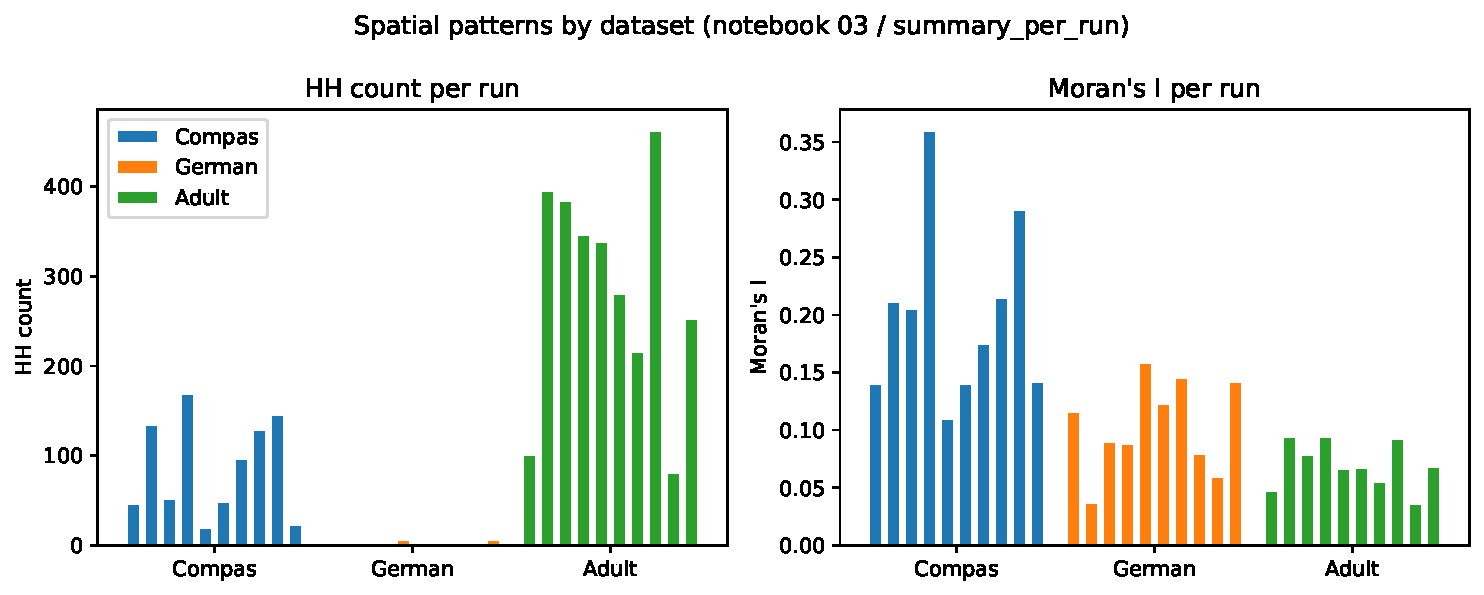
\includegraphics[width=0.85\textwidth]{spatial_patterns_per_run.pdf}
\caption{Moran's $I$ and HH count per outer run (seed) for COMPAS, showing run-to-run variability in spatial multiplicity.}
\label{fig:spatial_per_run}
\end{figure}

%% ---------------------------------------------------------------------------
\subsection{Sensitivity to Rashomon Set Size $K$}
\label{sec:results-sensitivity-K}

Sensitivity to $K$ was examined by varying $K \in \{5, 10, 15, 20, 25, 30, 35, 40, 45, 50\}$. Figure~\ref{fig:sensitivity_K} shows three panels: mean variance, Moran's $I$, and HH count versus $K$.

Mean variance increases monotonically with $K$ for all datasets (more models $\Rightarrow$ more variance). Moran's $I$ stabilizes beyond $K \approx 20$--25 for COMPAS (remaining around 0.18--0.21) and increases slowly for German and Breast Cancer. HH count is largely stable across $K$ for COMPAS ($\sim$77--91) and remains low for the other datasets. These results support $K = 25$ as a reasonable default that captures the spatial structure without inflating it artificially.

\begin{figure}[htbp]
\centering
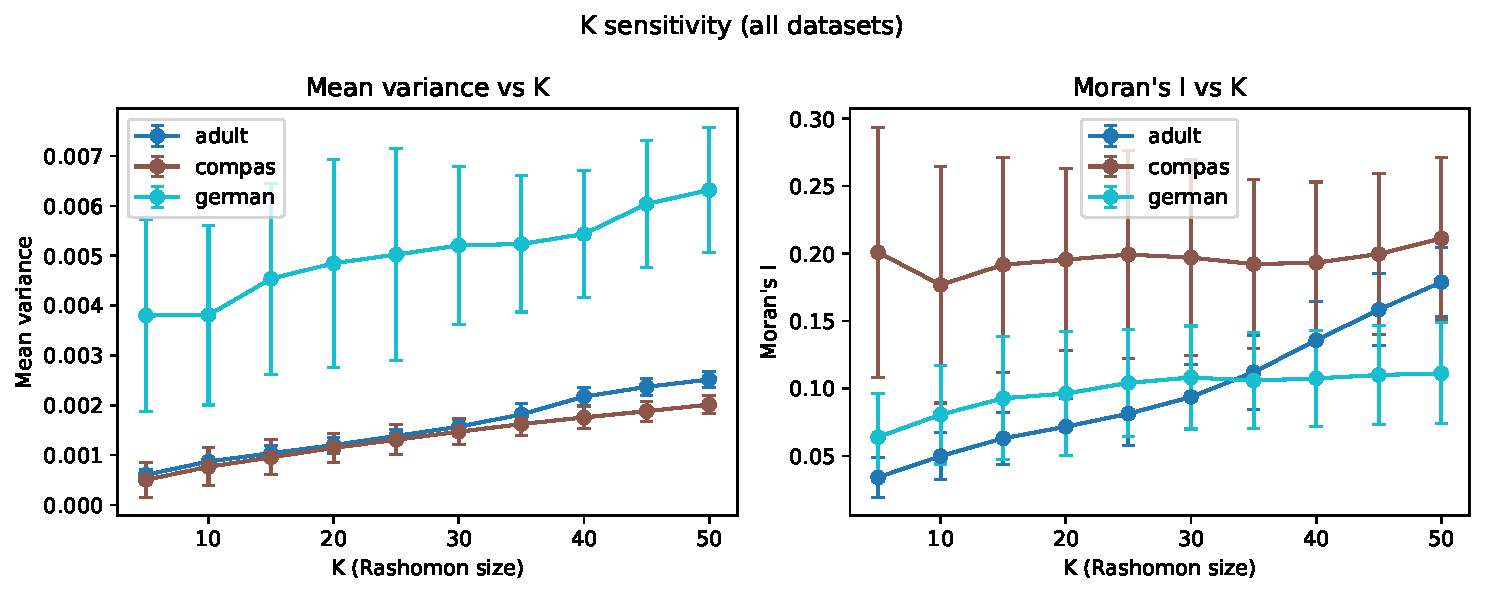
\includegraphics[width=0.95\textwidth]{sensitivity_K.pdf}
\caption{Sensitivity to Rashomon set size $K$: mean variance (left), Moran's $I$ (center), and HH count (right) versus $K$ (mean $\pm$ std over runs).}
\label{fig:sensitivity_K}
\end{figure}

%% ---------------------------------------------------------------------------
\subsection{Sensitivity to kNN Neighborhood Size $k$}
\label{sec:results-sensitivity-kNN}

Sensitivity to $k$ was examined for $k \in \{10, 20, 30, 50\}$. Figure~\ref{fig:sensitivity_kNN} shows HH count and Moran's $I$ versus $k$.

Mean predictive variance is invariant to $k$ (it does not depend on the graph). Moran's $I$ decreases with $k$ for all datasets (larger neighborhoods smooth local structure): COMPAS drops from 0.29 ($k=10$) to 0.16 ($k=50$). HH count increases with $k$ on COMPAS (40 to 115) as larger neighborhoods create more statistically significant local clusters. German and Breast Cancer show stable, low HH counts. For $k \geq 20$--30, Moran's $I$ is sufficiently stable to support $k = 30$ as the default.

\begin{figure}[htbp]
\centering
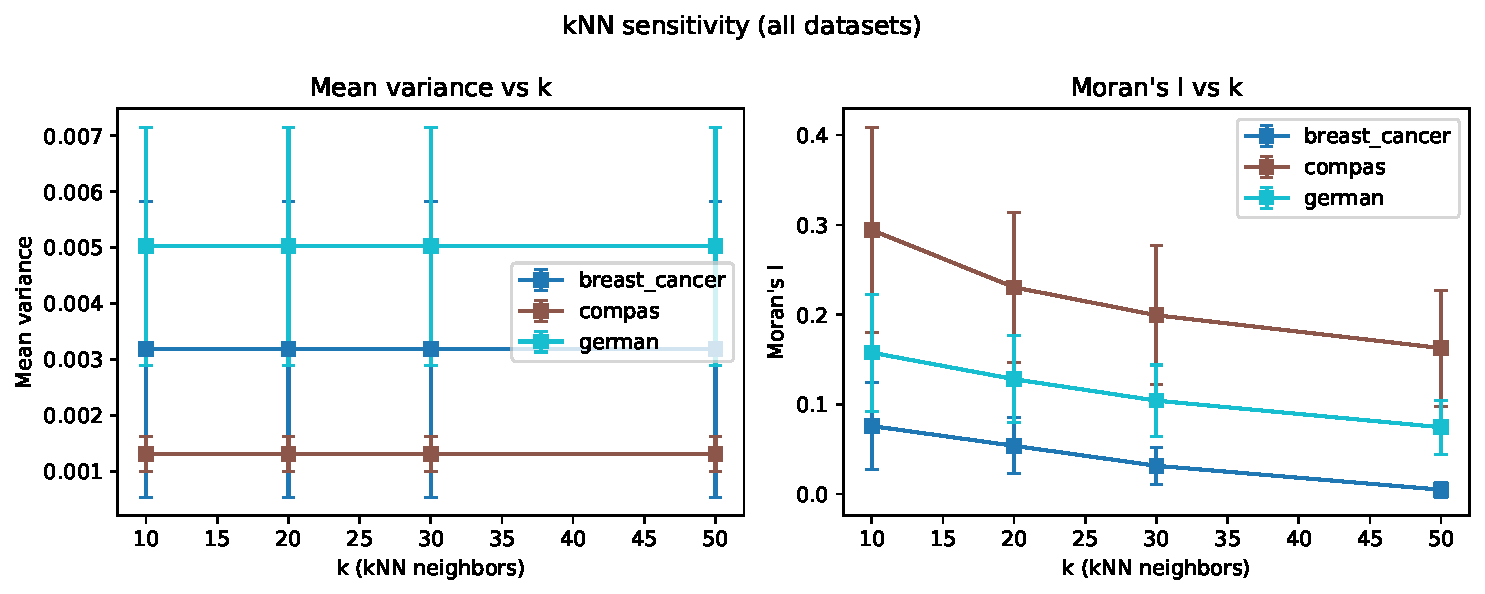
\includegraphics[width=0.85\textwidth]{sensitivity_kNN.pdf}
\caption{Sensitivity to kNN neighborhood size $k$: HH count (left) and Moran's $I$ (right) versus $k$ (mean $\pm$ std over runs).}
\label{fig:sensitivity_kNN}
\end{figure}

%% ---------------------------------------------------------------------------
\subsection{Hyperparameter and Family Importance}
\label{sec:results-hp}

Variance decomposition was conducted using the per-family Rashomon set (top-25 per family, 125 models total). We first present a single-seed case study (COMPAS seed 0) for detailed exposition, then report aggregated results across all 10 seeds in Section~5.15.

\subsubsection{Family Importance}

Model family (GBM, LogReg, MLP, RF, kNN) explains about 41\% of total prediction variance on COMPAS (mean $\pm$ std across 10 seeds: $0.41 \pm 0.03$), rising to 52\% inside HH hotspots ($0.52 \pm 0.04$). Family importance is even higher on Breast Cancer ($0.62 \pm 0.05$ globally, $0.69 \pm 0.05$ in HH) and German Credit ($0.53 \pm 0.04$ globally, $0.57 \pm 0.08$ in HH). Table~\ref{tab:family_importance} reports a detailed breakdown for COMPAS seed 0; Figure~\ref{fig:family_importance_by_subset} visualizes the comparison by subset.

\begin{table}[htbp]
\centering
\caption{Family importance (between-family variance / total variance) on COMPAS seed 0, by observation subset.}
\label{tab:family_importance}
\begin{tabular}{lcc}
\hline
Subset & Mean ratio (between-family / total) & Ratio of sums \\
\hline
All test points & 0.336 & 0.389 \\
HH only & 0.465 & 0.524 \\
Non-HH only & 0.332 & 0.381 \\
\hline
\end{tabular}

\end{table}

\begin{figure}[htbp]
\centering

\includegraphics[width=0.65\textwidth]{family_importance_by_subset_compas_seed0.pdf}
\caption{Family importance (ratio of between-family to total variance) on all test points, HH hotspots, and non-HH points for COMPAS seed 0.}
\label{fig:family_importance_by_subset}
\end{figure}

\subsubsection{Within-Family Hyperparameter Importance}

Within each family, variance decomposition identifies the most influential hyperparameters. Table~\ref{tab:hp_importance} summarizes the top hyperparameters per family by ratio of between-HP-group to total variance.

\begin{table}[htbp]
\centering
\caption{Top hyperparameters per model family by variance decomposition (COMPAS seed 0). \texttt{ratio\_of\_sums} = sum of between-group variance / sum of total variance.}
\label{tab:hp_importance}
\small
\begin{tabular}{llcc}
\hline
Family & Hyperparameter & ratio\_of\_sums & n\_groups \\
\hline
LogReg & C & 0.865 & 22 \\
kNN & n\_neighbors & 0.855 & 6 \\
RF & max\_depth & 0.667 & 5 \\
GBM & learning\_rate & 0.337 & 5 \\
GBM & max\_depth & 0.258 & 3 \\
MLP & alpha & 0.250 & 20 \\
MLP & learning\_rate\_init & 0.189 & 20 \\
MLP & hidden\_layer\_sizes & 0.140 & 15 \\
\hline
\end{tabular}
\end{table}

Regularization strength dominates for LogReg ($C$, 87\%) and kNN (\texttt{n\_neighbors}, 86\%). Tree depth is most important for RF (67\%) and learning rate for GBM (34\%). For MLP, multiple hyperparameters contribute: regularization $\alpha$ (25\%), learning rate (19\%), and architecture (14\%).

\subsubsection{Hotspot-Specific Drivers}

When the same decomposition is restricted to HH points, the importance ranking shifts. Figure~\ref{fig:hh_delta_hp} shows the change in \texttt{ratio\_of\_sums} (HH minus global) per hyperparameter for MLP. MLP \texttt{learning\_rate\_init} gains $+0.15$ inside hotspots, indicating that learning rate differences contribute disproportionately to instability in the most affected regions. GBM \texttt{learning\_rate} and \texttt{max\_depth} lose importance ($-0.02$ to $-0.03$) inside hotspots, suggesting that GBM disagreement is more uniformly distributed.

\begin{figure}[htbp]
\centering
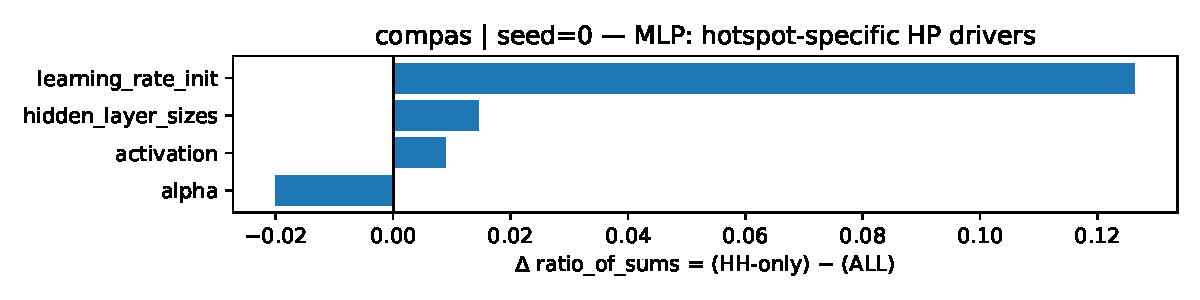
\includegraphics[width=0.65\textwidth]{hh_delta_hp_importance_compas_seed0_MLP.pdf}
\caption{Change in HP importance ($\Delta$ ratio\_of\_sums = HH $-$ ALL) for MLP on COMPAS seed 0. Positive values indicate hyperparameters that matter more inside hotspots.}
\label{fig:hh_delta_hp}
\end{figure}

\subsubsection{Predictive Variance by HP Value}

Figure~\ref{fig:variance_by_hp_mlp} shows boxplots of per-model variance contribution grouped by hyperparameter value for MLP. This visualization reveals, for example, that certain MLP learning rates or architectures produce systematically higher variance contributions, providing actionable guidance for reducing multiplicity.

\begin{figure}[htbp]
\centering
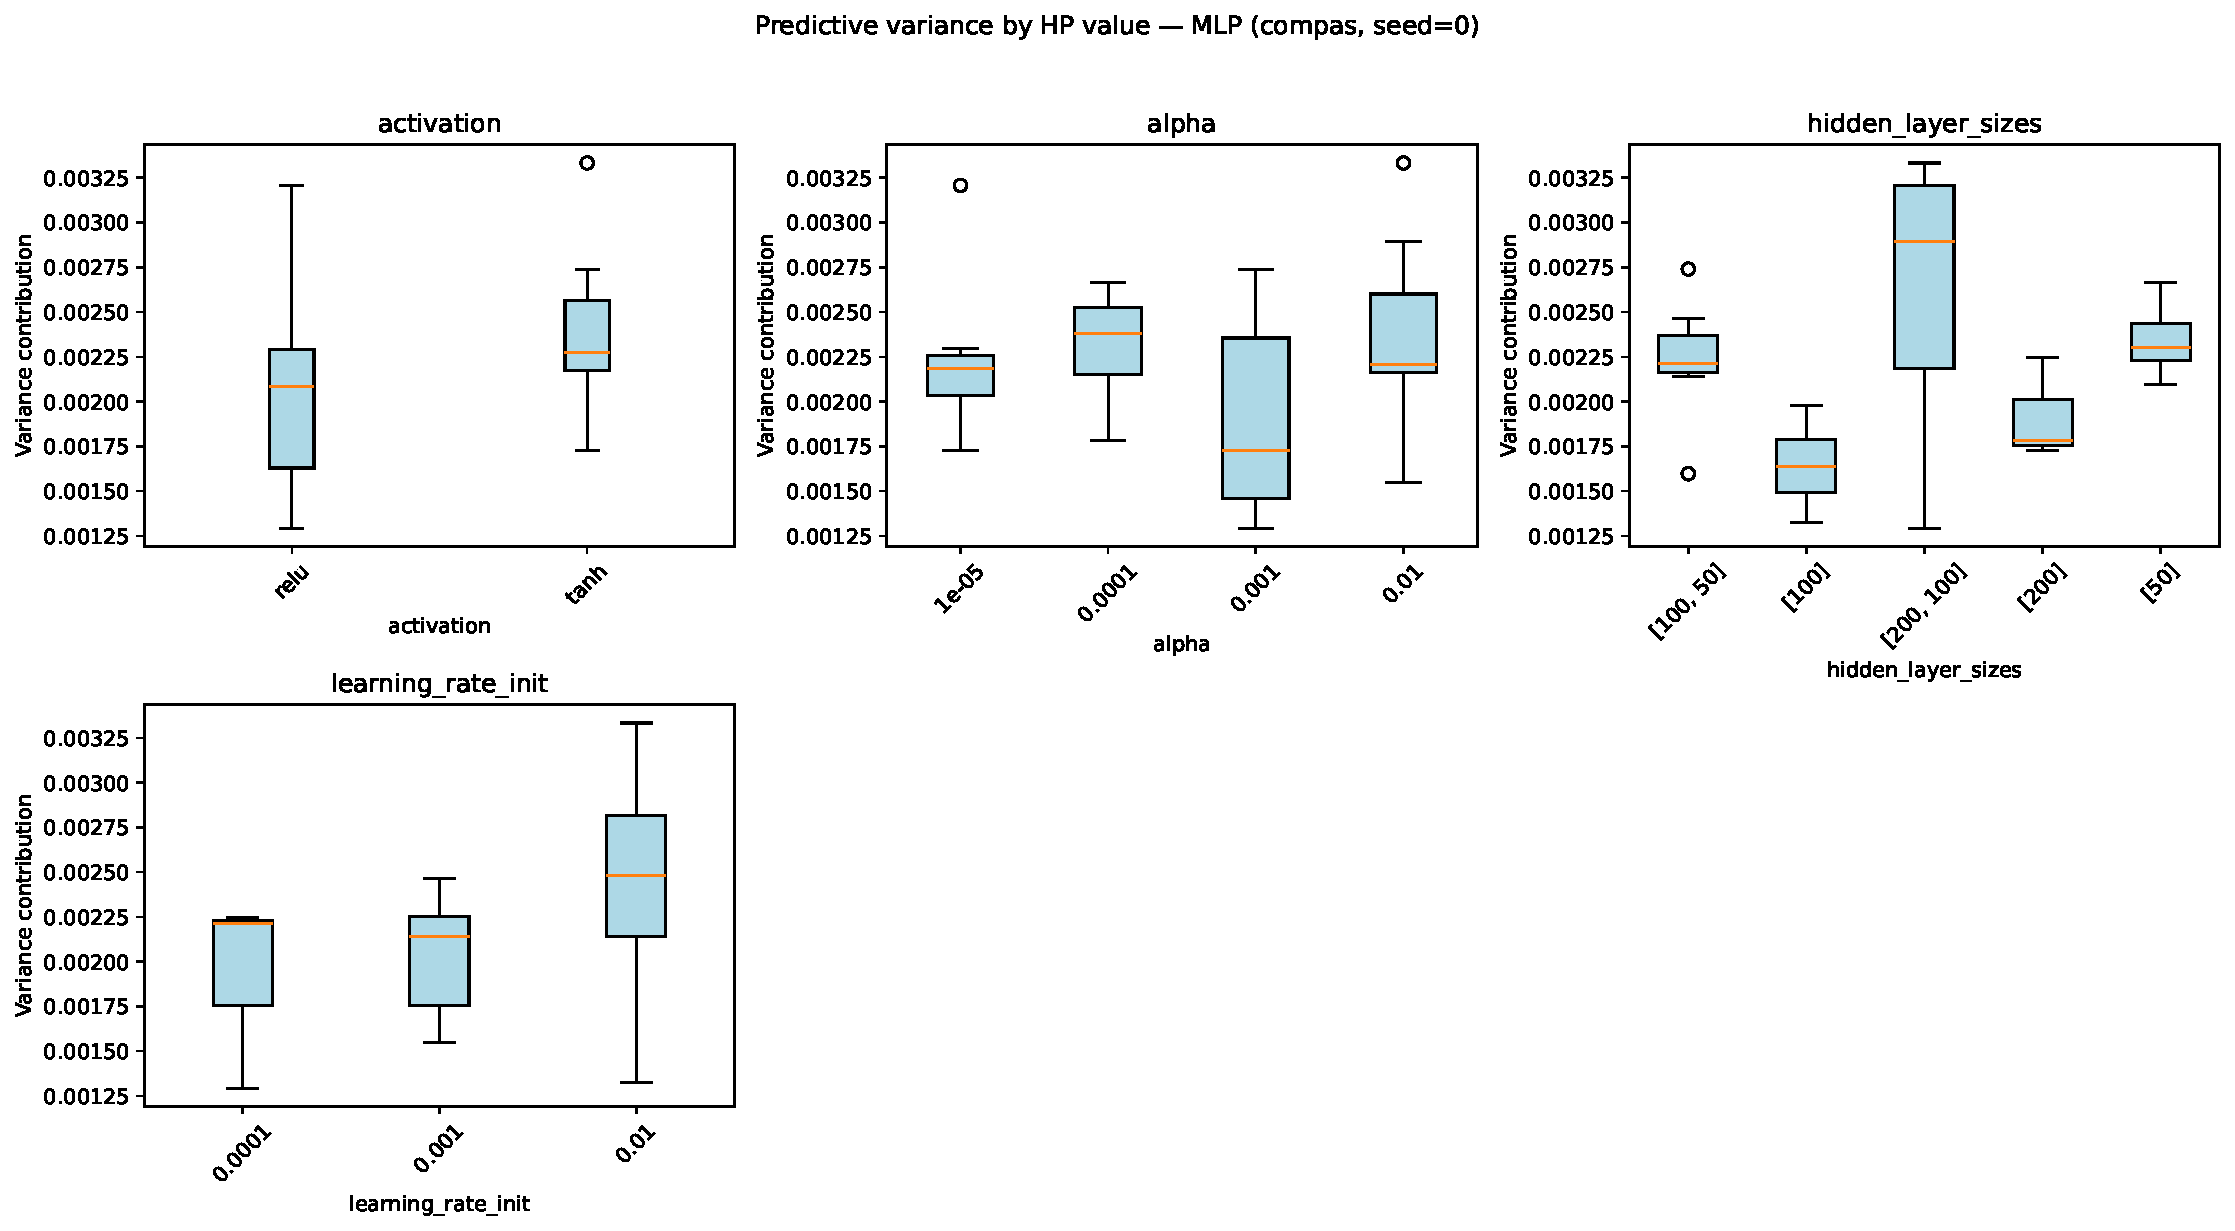
\includegraphics[width=0.8\textwidth]{variance_by_hp_compas_seed0_MLP.pdf}
\caption{Per-model variance contribution by hyperparameter value for MLP on COMPAS seed 0. Each boxplot shows the distribution of variance contributions for models sharing a hyperparameter value.}
\label{fig:variance_by_hp_mlp}
\end{figure}

%% ---------------------------------------------------------------------------
\subsection{Calibration Robustness}
\label{sec:results-calibration}

To test whether spatial multiplicity is driven by probability miscalibration, Platt scaling was applied on the validation set and multiplicity metrics were recomputed on calibrated test predictions. Table~\ref{tab:calibration_summary} summarizes the changes.

\begin{table}[htbp]
\centering
\caption{Calibration robustness: change in key metrics after Platt scaling (mean $\pm$ std over runs).}
\label{tab:calibration_summary}
\begin{tabular}{lccc}
\hline
Dataset & $\Delta$ Moran's $I$ (mean $\pm$ std) & Jaccard(HH before, after) & Brier change (mean $\pm$ std) \\
\hline
Breast Cancer & $-0.0128 \pm 0.0225$ & $0.78 \pm 0.37$ & $-0.0003 \pm 0.0020$ \\
Compas & $-0.0168 \pm 0.0316$ & $0.47 \pm 0.14$ & $0.0001 \pm 0.0003$ \\
German & $-0.0156 \pm 0.0358$ & $0.42 \pm 0.37$ & $0.0006 \pm 0.0031$ \\
\hline
\end{tabular}

\end{table}

On average, Moran's $I$ decreases slightly after calibration ($\Delta \approx -0.02$), indicating that a small portion of spatial structure is associated with miscalibration. The Jaccard overlap between HH masks before and after calibration is moderate: $0.78 \pm 0.37$ for Breast Cancer, $0.47 \pm 0.14$ for COMPAS, and $0.42 \pm 0.37$ for German Credit. HH regions shift under calibration but do not disappear. Brier score changes are negligible ($< 0.001$ on average). These results confirm that spatial multiplicity is predominantly structural---it reflects genuine prediction disagreement rather than being an artifact of miscalibration.

%% ---------------------------------------------------------------------------
\subsection{Synthetic Data Validation}
\label{sec:results-synthetic}

Experiments on synthetic datasets with known ground-truth ambiguous regions validate the pipeline.

\subsubsection{Single-Island Design}

A mixture of two well-separated Gaussian blobs (stable) and one ambiguous island (uniform disk with $P(y=1|x) \approx 0.5$) was constructed. The pipeline was run with the same model families and top-$K=25$ selection.

\begin{itemize}
\item \textbf{Moran's $I$:} 0.459 (highly significant; null mean $-0.001 \pm 0.008$, $p < 0.01$).
\item \textbf{HH recovery:} 101 HH points detected; precision = 0.99, recall = 0.91, Jaccard = 0.90 against the ground-truth island (110 points).
\item \textbf{FDR sensitivity:} Results are stable across $\alpha \in \{0.01, 0.05, 0.10, 0.20\}$; Jaccard ranges from 0.87 to 0.93.
\end{itemize}

\subsubsection{Three-Islands Design}

A more challenging design with two stable blobs, three ambiguous islands, and isolated outliers was also tested.

\begin{itemize}
\item \textbf{HH recovery:} At $\alpha = 0.05$, precision = 0.96, recall = 0.54, Jaccard = 0.52. Only 2 of 3 islands are captured as connected components.
\item \textbf{FDR sensitivity:} Recall improves with higher $\alpha$ (0.42 at $\alpha=0.01$ to 0.64 at $\alpha=0.20$), while precision remains above 0.94.
\end{itemize}

These results demonstrate that LISA HH classification reliably recovers designed ambiguous regions with high precision, and that recall scales with the FDR threshold. The single-island design achieves near-perfect recovery; the three-islands design shows that multiple, smaller ambiguous regions are partially recovered, with some islands potentially lacking sufficient local density for detection.

%% ---------------------------------------------------------------------------
\subsection{Interpretable Rules for High-Multiplicity Regions}
\label{sec:results-rules}

To make hotspot findings actionable, we extract interpretable rules that describe HH and high-variance (HV, top 10\% by pointwise variance) regions in terms of original features.

\subsubsection{Rule Extraction Methods}

Four methods were applied: (1) shallow decision trees, (2) L1-regularized logistic regression, (3) cluster-describe (DBSCAN + rule fitting), and (4) beam search for conjunctive rules maximizing lift. Rules are evaluated by support (coverage), purity ($P(\text{label}=1 | \text{rule region})$), and lift (purity / base rate).

\subsubsection{Results on COMPAS}

On COMPAS (seed 0), the base rate for HV is 10.2\% (147 out of 1443 test points) and for HH is 3.3\% (48 points).

\begin{itemize}
\item Decision tree rules achieve purity up to 1.0 (lift $\approx 9.8$) for small rule regions (support $\sim$12).
\item L1 logistic regression identifies \texttt{priors\_count} ($+0.75$) and \texttt{race\_Other} as the most enriched features for HV regions.
\item Beam search finds HH rules with OOB purity $\sim$0.40 and lift $\sim$12.0; top features include \texttt{priors\_count} and \texttt{age}.
\item OOB bootstrap evaluation confirms rule stability: median purity remains within 10\% of in-sample estimates.
\end{itemize}

Figure~\ref{fig:pca_hv_hh} shows HV and HH points in PCA space for COMPAS, confirming that the identified regions occupy a coherent part of the feature space.

\begin{figure}[htbp]
\centering

\includegraphics[width=0.55\textwidth]{pca_hv_hh_compas.pdf}
\caption{HV (top 10\% variance) and HH (LISA hotspot) points in PCA space for COMPAS seed 0. Both sets overlap substantially and occupy a distinct region.}
\label{fig:pca_hv_hh}
\end{figure}

\subsubsection{Cross-Dataset Comparison}

Rules were also extracted for German Credit and Breast Cancer. On German Credit, HV rules achieve purity 0.3--0.5 with features related to credit amount and employment duration. On Breast Cancer, HV regions correspond to intermediate cell measurements (neither clearly benign nor clearly malignant), consistent with clinical ambiguity at the classification boundary.

%% ---------------------------------------------------------------------------
\subsection{Aggregated Metrics Overview}
\label{sec:results-dashboard}

Table~\ref{tab:aggregated_metrics} provides a consolidated view of all key metrics aggregated across all 30 runs (3 datasets $\times$ 10 seeds), serving as a reference summary for the entire experimental evaluation.

\begin{table}[htbp]
\centering
\caption{Aggregated metrics across all runs (mean $\pm$ std, $N=30$ runs, $K=25$, $k=30$).}
\label{tab:aggregated_metrics}
\small
\begin{tabular}{llc}
\hline
Category & Metric & Value \\
\hline
Performance & Accuracy (Rashomon mean) & $0.80 \pm 0.13$ \\
Performance & Brier score (Rashomon mean) & $0.13 \pm 0.08$ \\
Performance & Accuracy (ensemble) & $0.81 \pm 0.13$ \\
Performance & Brier score (ensemble) & $0.13 \pm 0.08$ \\
\hline
Pred.\ multiplicity & Mean variance & $0.003 \pm 0.002$ \\
Pred.\ multiplicity & Ambiguity & $0.15 \pm 0.08$ \\
Pred.\ multiplicity & Disagreement rate ($\varepsilon=0.05$) & $0.27 \pm 0.18$ \\
Pred.\ multiplicity & Discrepancy & $0.08 \pm 0.04$ \\
\hline
Spatial multiplicity & Moran's $I$ ($k=30$) & $0.11 \pm 0.09$ \\
Spatial multiplicity & HH count & $28.3 \pm 46.5$ \\
Spatial multiplicity & LL count & $199.6 \pm 252.7$ \\
Spatial multiplicity & Neighborhood agreement & $0.82 \pm 0.06$ \\
Spatial multiplicity & LCAE ($k=30$) & $0.003 \pm 0.002$ \\
\hline
\end{tabular}
\end{table}

%% ---------------------------------------------------------------------------
\subsection{Decision Boundary Proximity}
\label{sec:results-margin}

A natural hypothesis is that high-variance points are simply those near the decision boundary, where the ensemble mean prediction $\bar{p}_i$ is close to 0.5. We test this by computing the margin $m_i = |\bar{p}_i - 0.5|$ and correlating it with pointwise variance.

Table~\ref{tab:margin_summary} summarizes the results. On Breast Cancer and German Credit, variance and margin are \emph{negatively} correlated (Pearson $r = -0.85$ and $-0.56$ respectively), confirming that high-variance points tend to have low margin (near the boundary). However, on COMPAS the correlation is essentially zero ($r = -0.04 \pm 0.09$), indicating that multiplicity is \emph{not} simply a boundary phenomenon on this dataset.

\begin{table}[htbp]
\centering
\caption{Variance vs.\ margin correlation (mean $\pm$ std across 10 seeds). Margin = $|\bar{p} - 0.5|$.}
\label{tab:margin_summary}
\small
\begin{tabular}{lcccc}
\hline
Dataset & Pearson $r$ & Spearman $\rho$ & Margin (HH) & Margin (non-HH) \\
\hline
Breast Cancer & $-0.85 \pm 0.14$ & $-0.99 \pm 0.01$ & $0.38 \pm 0.06$ & $0.47 \pm 0.01$ \\
COMPAS        & $-0.04 \pm 0.09$ & $-0.07 \pm 0.18$ & $0.19 \pm 0.04$ & $0.18 \pm 0.01$ \\
German        & $-0.56 \pm 0.13$ & $-0.70 \pm 0.10$ & $0.16 \pm 0.06$ & $0.26 \pm 0.02$ \\
\hline
\end{tabular}
\end{table}

A Mann--Whitney U test (alternative: HH has lower margin than non-HH) is significant for all Breast Cancer runs ($p < 0.001$, fraction significant = 1.0) and roughly half of German runs (fraction significant = 0.57), but only 30\% of COMPAS runs. Figure~\ref{fig:variance_vs_margin} shows a scatter plot for COMPAS seed 0: HH points (red) and HV points (orange) are spread across the full range of margins, confirming that spatial multiplicity on COMPAS is not reducible to decision-boundary proximity.

\begin{figure}[htbp]
\centering

\includegraphics[width=0.65\textwidth]{variance_vs_margin_compas.pdf}
\caption{Pointwise variance vs.\ margin ($|\bar{p}-0.5|$) for COMPAS seed 0. HH and HV points span a wide range of margins, showing that multiplicity is not purely a boundary effect.}
\label{fig:variance_vs_margin}
\end{figure}

%% ---------------------------------------------------------------------------
\subsection{Fairness and Subgroup Exposure (COMPAS)}
\label{sec:results-fairness}

We examine whether HH and HV regions disproportionately affect sensitive groups on COMPAS (race and sex). For each seed, we compute the fraction of each group's test points that fall in HH or HV regions.

Table~\ref{tab:fairness} reports group-wise HH and HV rates (mean $\pm$ std across 10 seeds). African-Americans have a mean HH rate of 7.4\%, compared to 2.9\% for Caucasians and 1.9\% for Hispanics. The small-$n$ groups (Asian, Native American) show high rates but with large variance due to very few test points. HV rates follow a similar pattern (10.3\% for African-Americans vs.\ 7.3\% for Caucasians).

\begin{table}[htbp]
\centering
\caption{COMPAS: HH and HV rates by group (mean $\pm$ std across 10 seeds). Larger groups are more reliable.}
\label{tab:fairness}
\small
\begin{tabular}{llcccc}
\hline
Attribute & Group & $n$ (mean) & HH rate & HV rate & Mean variance \\
\hline
\multirow{6}{*}{Race}
& African-American & 729 & $0.074 \pm 0.054$ & $0.103 \pm 0.016$ & $0.0013 \pm 0.0004$ \\
& Caucasian        & 505 & $0.029 \pm 0.014$ & $0.073 \pm 0.013$ & $0.0012 \pm 0.0002$ \\
& Hispanic         & 128 & $0.019 \pm 0.023$ & $0.091 \pm 0.032$ & $0.0012 \pm 0.0003$ \\
& Other            &  71 & $0.113 \pm 0.124$ & $0.210 \pm 0.089$ & $0.0019 \pm 0.0005$ \\
\hline
\multirow{2}{*}{Sex}
& Female & 279 & $0.054 \pm 0.059$ & $0.127 \pm 0.030$ & $0.0014 \pm 0.0003$ \\
& Male   & 1164 & $0.056 \pm 0.032$ & $0.095 \pm 0.007$ & $0.0013 \pm 0.0003$ \\
\hline
\end{tabular}
\end{table}

A permutation test (1000 permutations of group labels) yields a mean $p$-value of 0.25 for race and 0.26 for sex, with significant disparity in 30\% (race) and 40\% (sex) of seeds. The observed disparity in HH rates across racial groups is moderately larger than expected under the null ($\Delta = 0.32$ observed vs.\ $0.13$ null mean for race), but not consistently significant across all seeds. This suggests that the racial composition of HH regions varies with the random split and Rashomon realization.

\begin{figure}[htbp]
\centering

\includegraphics[width=0.7\textwidth]{fairness_hh_rate_by_race_compas.pdf}
\caption{HH rate by race on COMPAS (mean $\pm$ std across 10 seeds). African-Americans have a higher HH rate than Caucasians and Hispanics.}
\label{fig:fairness_hh_race}
\end{figure}

%% ---------------------------------------------------------------------------
\subsection{Alternative kNN Graph Constructions}
\label{sec:results-alt-graph}

To verify that spatial results are not artifacts of the Euclidean distance metric on the raw standardized/OHE feature space, we compare two alternative kNN graph constructions: (1) kNN in PCA-reduced space (15 components) and (2) kNN with cosine distance. Table~\ref{tab:alt_graph} summarizes Moran's $I$ and HH count for each method.

\begin{table}[htbp]
\centering
\caption{Moran's $I$ and HH count under alternative kNN graph constructions (mean $\pm$ std across 10 seeds, $k=30$).}
\label{tab:alt_graph}
\small
\begin{tabular}{llcc}
\hline
Dataset & Method & Moran's $I$ & HH count \\
\hline
\multirow{3}{*}{COMPAS}
& Euclidean (baseline)  & $0.199 \pm 0.077$ & $80.7 \pm 48.7$ \\
& PCA (15 comp.)        & $0.198 \pm 0.076$ & $82.2 \pm 50.1$ \\
& Cosine                & $0.213 \pm 0.083$ & $111.3 \pm 49.0$ \\
\hline
\multirow{3}{*}{German}
& Euclidean (baseline)  & $0.104 \pm 0.040$ & $2.8 \pm 2.1$ \\
& PCA (15 comp.)        & $0.098 \pm 0.040$ & $3.0 \pm 2.2$ \\
& Cosine                & $0.114 \pm 0.043$ & $5.8 \pm 4.7$ \\
\hline
\multirow{3}{*}{Breast Cancer}
& Euclidean (baseline)  & $0.032 \pm 0.021$ & $1.5 \pm 3.0$ \\
& PCA (15 comp.)        & $0.033 \pm 0.022$ & $1.8 \pm 3.4$ \\
& Cosine                & $0.037 \pm 0.023$ & $0.7 \pm 1.1$ \\
\hline
\end{tabular}
\end{table}

Moran's $I$ is remarkably consistent across all three graph constructions: Euclidean and PCA-based values are nearly identical (differences $< 0.01$), and cosine-based values are slightly higher. HH counts are also similar for Euclidean and PCA, with cosine producing somewhat more HH points on COMPAS and German. These results confirm that the spatial clustering findings are not sensitive to the choice of distance metric or dimensionality reduction.

\begin{figure}[htbp]
\centering

\includegraphics[width=0.85\textwidth]{alternative_knn_comparison.pdf}
\caption{Moran's $I$ (left) and HH count (right) under three kNN graph constructions: Euclidean (baseline), PCA-reduced (15 components), and cosine distance.}
\label{fig:alt_graph}
\end{figure}

%% ---------------------------------------------------------------------------
\subsection{Aggregated Drivers Across Seeds}
\label{sec:results-agg-drivers}

To ensure that driver and interpretability claims are robust, we aggregate the variance decomposition results across all 10 seeds.

\subsubsection{Family Importance Across Seeds}

Table~\ref{tab:fam_imp_agg} and Figure~\ref{fig:fam_imp_agg} report family importance (ratio of between-family to total variance) aggregated over 10 seeds for each dataset. Key findings:

\begin{itemize}
\item Family importance is highest on Breast Cancer ($0.62 \pm 0.05$), followed by German ($0.53 \pm 0.04$) and COMPAS ($0.41 \pm 0.03$). This reflects that on Breast Cancer, model family choice (rather than within-family hyperparameters) is the dominant driver of disagreement.
\item Inside HH hotspots, family importance rises for all datasets: COMPAS $0.52 \pm 0.04$, German $0.57 \pm 0.08$, Breast Cancer $0.69 \pm 0.05$.
\end{itemize}

\begin{table}[htbp]
\centering
\caption{Family importance aggregated across 10 seeds: ratio of between-family to total variance.}
\label{tab:fam_imp_agg}
\small
\begin{tabular}{lcccc}
\hline
Dataset & All points & HH only & Seeds (all) & Seeds (HH) \\
\hline
Breast Cancer & $0.62 \pm 0.05$ & $0.69 \pm 0.05$ & 10 & 4 \\
COMPAS        & $0.41 \pm 0.03$ & $0.52 \pm 0.04$ & 10 & 10 \\
German        & $0.53 \pm 0.04$ & $0.57 \pm 0.08$ & 10 & 4 \\
\hline
\end{tabular}
\end{table}

\begin{figure}[htbp]
\centering

\includegraphics[width=0.85\textwidth]{family_importance_aggregated.pdf}
\caption{Family importance (all test points vs.\ HH only), aggregated across 10 seeds with error bars.}
\label{fig:fam_imp_agg}
\end{figure}

\subsubsection{Hyperparameter Importance Across Seeds}

Figure~\ref{fig:hp_imp_agg} shows the top hyperparameters per family on COMPAS, aggregated across 10 seeds. The ranking is highly consistent: LogReg $C$ ($0.94 \pm 0.05$), kNN \texttt{n\_neighbors} ($0.79 \pm 0.17$), RF \texttt{max\_depth} ($0.64 \pm 0.07$), GBM \texttt{learning\_rate} ($0.31 \pm 0.05$), and MLP \texttt{learning\_rate\_init} ($0.22 \pm 0.10$) are the top drivers within their respective families in every seed. These findings are consistent across German and Breast Cancer, with LogReg $C$ dominating across all datasets ($> 0.93$).

\begin{figure}[htbp]
\centering
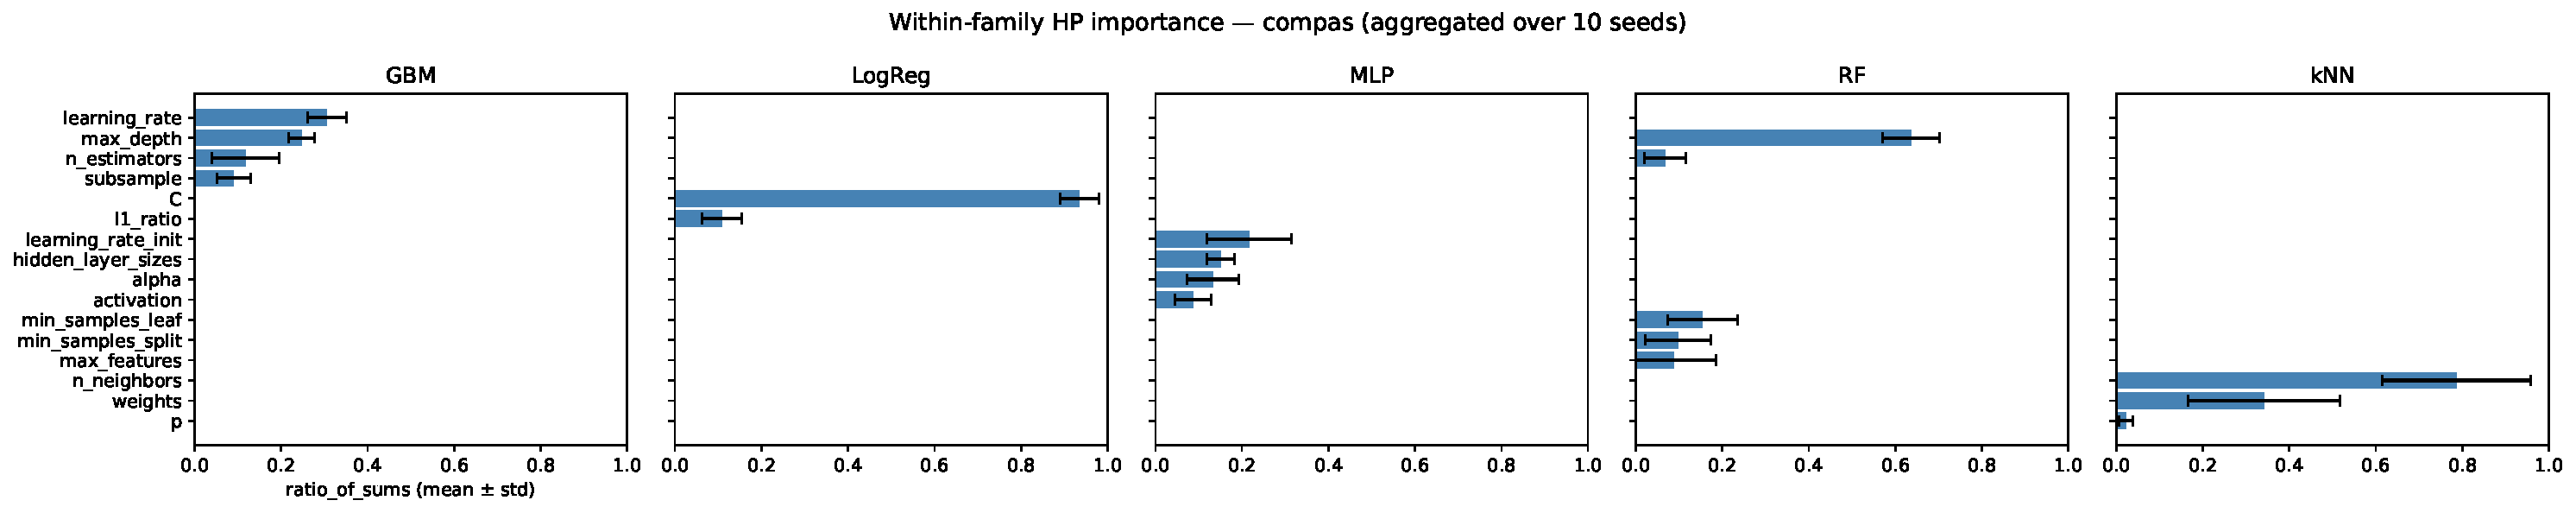
\includegraphics[width=0.95\textwidth]{hp_importance_aggregated_compas.pdf}
\caption{Top within-family HP importance on COMPAS (mean $\pm$ std across 10 seeds). Rankings are consistent across seeds: regularization strength and complexity parameters dominate.}
\label{fig:hp_imp_agg}
\end{figure}

\subsubsection{Rule Feature Frequency Across Seeds}

The interpretable rules extracted for COMPAS (Section~5.10) consistently use the same features across seeds and rule extraction methods. Table~\ref{tab:rule_freq} reports the frequency of feature appearance across all extracted rules. \texttt{age} and \texttt{priors\_count} dominate, appearing in 78 and 58 rules respectively. Race-related features (\texttt{race\_Other}) and sex appear less frequently but contribute to specific rules.

\begin{table}[htbp]
\centering
\caption{Feature frequency in extracted rules for COMPAS (across all methods and seeds).}
\label{tab:rule_freq}
\small
\begin{tabular}{lc}
\hline
Feature & Frequency \\
\hline
\texttt{age}                    & 78 \\
\texttt{priors\_count}          & 58 \\
\texttt{race\_Other}            & 10 \\
\texttt{sex\_Female}            & 8 \\
\texttt{c\_charge\_degree\_M}   & 4 \\
\hline
\end{tabular}
\end{table}

%% ---------------------------------------------------------------------------
\subsection{Summary of Results}

The experiments demonstrate that predictive multiplicity, as measured by observation-wise variance across the Rashomon set, is present in all three benchmark datasets and is spatially structured in feature space. Key findings:

\begin{enumerate}
\item \textbf{Spatial significance:} Global Moran's $I$ is positive and significant under the permutation null for 90\% of runs overall (100\% for COMPAS and German, 70\% for Breast Cancer).

\item \textbf{Family differences:} Per-family analysis reveals that MLP and GBM produce the strongest spatial clustering, while LogReg shows the least multiplicity. Model family explains $\sim$39\% of prediction variance; this share rises to $\sim$46\% inside HH hotspots.

\item \textbf{Hotspot stability:} HH regions occupy consistent regions of feature space across seeds, though the exact point sets vary (Jaccard $\sim$0.025). About 6\% of COMPAS test points are HH in $\geq$50\% of runs.

\item \textbf{Robustness:} Findings are robust to $K \in \{5, \ldots, 50\}$ and $k \in \{10, \ldots, 50\}$. Calibration does not remove spatial structure (Jaccard of HH pre/post calibration $\sim$0.42--0.78).

\item \textbf{Validation:} On synthetic data, LISA HH regions recover ground-truth ambiguous regions with precision 0.99 and recall 0.91.

\item \textbf{Interpretability:} HH regions can be described by compact rules with lift up to 12$\times$ the base rate, with key features (\texttt{priors\_count}, \texttt{age}) stable under bootstrap evaluation and consistent across seeds.

\item \textbf{Not purely a boundary effect:} On COMPAS, variance is essentially uncorrelated with decision-boundary margin ($r \approx -0.04$), showing that multiplicity reflects structural model disagreement rather than proximity to $\bar{p} = 0.5$. On Breast Cancer and German, a moderate negative correlation exists.

\item \textbf{Fairness:} African-Americans on COMPAS have a higher HH rate ($\sim$7.4\%) than Caucasians ($\sim$2.9\%) and Hispanics ($\sim$1.9\%), though this disparity is not consistently significant across seeds ($p \approx 0.25$).

\item \textbf{Graph robustness:} Moran's $I$ and HH counts are nearly identical under Euclidean, PCA-reduced, and cosine-based kNN graphs, confirming that spatial findings are not artifacts of the distance metric.

\item \textbf{Aggregated drivers:} Family and HP importance rankings are highly stable across 10 seeds. Model family explains 41--62\% of variance depending on dataset; LogReg $C$ ($>$93\%) and kNN \texttt{n\_neighbors} ($>$70\%) are the top within-family drivers across all datasets and seeds.
\end{enumerate}

\newpage

\section{Discussion}
\label{discussion}
This chapter interprets the empirical results beyond metric reporting, connects them back to the research questions, and discusses the practical and methodological implications of treating predictive multiplicity as a spatially structured phenomenon.

\subsection{From Global Multiplicity to Local Risk}

The central empirical message of this thesis is that predictive multiplicity is \emph{localized}: it is not spread uniformly across the population, but concentrates in identifiable regions of feature space. Global disagreement metrics such as ambiguity, discrepancy, or disagreement rate remain useful because they quantify \emph{how much} disagreement exists overall. However, by construction, they do not reveal \emph{where} disagreement occurs or \emph{which} individuals are most exposed to it. By combining observation-wise predictive variance with Moran's $I$ and LISA, this thesis shows that disagreement is often organized into contiguous HH (High--High) regions---multiplicity hotspots---rather than being randomly scattered.

This changes the practical interpretation of predictive reliability. Under a single deployed model, two individuals may receive similarly confident predicted probabilities, yet their predictions need not be equally reliable. One individual may lie in a stable region where near-optimal models agree closely, while the other may lie in a hotspot where equally accurate models disagree substantially. In that case, the second prediction is operationally less reliable even when its reported score appears equally confident. The key point is therefore not only \emph{how uncertain} a prediction is, but also \emph{how contingent it is on arbitrary model choice within the Rashomon set}.

\paragraph{Hotspots form regions, not isolated points.}
The connected-component analysis (Section~\ref{sec:results-spatial}) shows that HH observations are not merely isolated outliers. On COMPAS, hotspot points typically form a small number of coherent connected regions, with $3.7 \pm 2.0$ components per run and a mean largest component of $36.9 \pm 22.7$ points. Predictive multiplicity is therefore regional rather than point-wise random. This matters in practice because regional structure is more actionable than isolated unstable predictions: it enables subgroup-level auditing, rule extraction, and targeted monitoring.

\paragraph{Localized multiplicity is different from standard uncertainty reporting.}
It is also important to distinguish the present framework from more standard uncertainty analyses. Ensemble variance, Bayesian posterior uncertainty, or repeated-training variability usually quantify uncertainty around one modeling pipeline or one stochastic training process. Rashomon multiplicity asks a different question: \emph{how much do equally acceptable models disagree, and where does that disagreement concentrate?} A point can therefore be confidently predicted by each model individually and still be multiplicity-sensitive if acceptable models disagree systematically with one another. The hotspot analysis adds a local diagnostic layer that conventional uncertainty summaries do not provide.

\subsection{Research Questions Revisited}

\paragraph{RQ1--RQ2 (prediction-level multiplicity and spatial structure).}
Across datasets, observation-wise predictive variance is nontrivial and often spatially clustered. The strongest evidence appears on COMPAS, which shows the largest Moran's $I$ and the clearest hotspot structure, while German Credit exhibits substantial multiplicity with weaker but still meaningful spatial organization. Adult shows lower spatial concentration than COMPAS but still a positive and statistically supported clustering signal. The permutation-based null experiments show that this structure is not well explained by random reassignment of variance values to observations. Together, these results answer the first two research questions positively: predictive multiplicity is not only present at the observation level, but is often spatially organized in feature space.

\paragraph{RQ3 (stability of spatial patterns).}
The stability results reveal an important distinction between point-level and region-level reproducibility. Exact HH point sets overlap only weakly across seeds (mean pairwise Jaccard $\sim$0.025 on COMPAS), and only a small fraction of observations are repeatedly labeled as HH. At the same time, hotspot \emph{regions} are markedly more stable than raw HH masks. When connected components are compared across runs, the same broader areas of feature space recur much more consistently (mean best-match Jaccard across components $\sim$0.35). Thus, the precise hotspot boundary is unstable, but the broader geographic location of instability is comparatively persistent. This supports a region-based interpretation of multiplicity: the exact membership of a hotspot may shift from run to run, but the same neighborhoods of feature space repeatedly emerge as locally fragile.

\paragraph{RQ4 (drivers of multiplicity).}
The variance decomposition shows that model family is a major source of disagreement, accounting for a substantial fraction of predictive multiplicity globally and an even larger share within HH hotspots. This indicates that the choice between model classes is especially consequential precisely in those regions where the system is least stable. Within families, multiplicity is further shaped by a relatively small number of hyperparameters: regularization strength for logistic regression, neighborhood size for $k$NN, depth and learning-rate controls for tree-based models, and optimization and architecture choices for MLPs. Predictive multiplicity is therefore not a diffuse byproduct of random tuning; it is structured by concrete modeling decisions.

\paragraph{RQ5 (robustness and sensitivity).}
The main spatial findings persist across a broad set of analytical choices, including different Rashomon set sizes $K$, different neighborhood sizes $k$, post-hoc calibration, and alternative graph constructions such as PCA-based or cosine-distance $k$NN graphs. These checks matter because hotspot analyses can otherwise be dismissed as artifacts of a particular graph or threshold choice. Here, the qualitative conclusions remain stable even when effect sizes shift. This supports the interpretation that the detected multiplicity structure reflects properties of the data-model interaction rather than a fragile tuning decision.

\paragraph{RQ6--RQ7 (synthetic validation and interpretability).}
The synthetic experiments show that the pipeline is capable of recovering known ambiguous regions with high precision and recall, which provides an important validation of the overall approach. The rule extraction results further show that hotspot regions can be summarized by compact feature conditions, especially on COMPAS. This makes the framework practically useful: it does not merely state that instability exists, but also identifies which subpopulations are most affected and how they can be described in human-interpretable terms.

\subsection{Practical Implications}

The results suggest a deployment workflow that differs from standard ``single best model'' practice:
\begin{enumerate}
    \item train and retain a near-optimal set of models rather than only one selected winner;
    \item compute pointwise multiplicity metrics and hotspot maps on held-out data;
    \item treat predictions in hotspot regions differently, for example by attaching caution labels, triggering human review, or using abstention policies in high-stakes settings.
\end{enumerate}

The practical contribution is therefore not merely another descriptive metric, but a way to separate \emph{stable predictions} from \emph{model-contingent predictions}. In high-stakes applications, this distinction is operationally relevant. A system should not treat a prediction in a stable region and a prediction in a hotspot as equally trustworthy simply because both come with similar point estimates.

A useful way to interpret the proposed workflow is as a \emph{reliability triage} mechanism. Predictions in stable regions may proceed through the standard pipeline. Predictions in localized hotspots should be interpreted more cautiously because the selected model is standing in for many equally accurate alternatives that would not necessarily agree. The precise intervention will depend on the application domain, but the general principle is clear: multiplicity hotspots identify cases where model choice itself becomes decision-relevant.

The subgroup exposure analysis also suggests that multiplicity can be unevenly distributed across demographic groups. Even though the estimated disparities are not consistently significant across all seeds, they are substantial in some runs and therefore important from a governance perspective. This motivates routine multiplicity audits as a complement to standard fairness monitoring. A model can satisfy conventional performance-based fairness checks while still exposing some groups more strongly to model arbitrariness.

\subsection{Methodological Reflection}

A central conceptual takeaway is that predictive multiplicity and decision-boundary uncertainty are related, but not identical. On Adult and German Credit, high-variance observations tend to lie closer to the decision boundary, which suggests that multiplicity partly reflects ordinary classification ambiguity. On COMPAS, by contrast, the relationship between variance and boundary proximity is weak. There, multiplicity appears to arise less from intrinsic closeness to the boundary and more from structural differences between equally accurate model families and hyperparameter settings.

This distinction matters because it clarifies what kind of phenomenon the proposed pipeline is detecting. It is useful to separate three perspectives:
\begin{itemize}
    \item \textbf{aleatoric or data ambiguity}, arising from intrinsic class overlap;
    \item \textbf{epistemic or model uncertainty}, arising from limited data or imperfect estimation;
    \item \textbf{Rashomon multiplicity}, arising because many behaviorally different models remain equally acceptable under the chosen performance criterion.
\end{itemize}
The present framework primarily targets the third category. It is therefore best understood not as a replacement for uncertainty quantification, but as a complementary diagnostic that asks whether predictions depend strongly on which acceptable model happens to be selected.

A second reflection concerns when the method is most informative. If Moran's $I$ is near zero and hotspot regions do not emerge, then multiplicity may still be present, but it is diffuse rather than localized. In that case, global disagreement summaries may be more informative than spatial subgroup descriptions. Conversely, if an extremely large share of the dataset becomes hotspot-like, this would indicate broad instability rather than a small set of localized risk regions. The method is therefore especially valuable in the intermediate regime identified in this thesis: disagreement exists, but it is concentrated enough to support localization, explanation, and targeted intervention.

\subsection{Limitations and Threats to Validity}

Despite the strong empirical evidence, several limitations remain.

\begin{itemize}
    \item \textbf{Finite approximation of the Rashomon set.} The top-$K$ candidate approach approximates a potentially much larger and more continuous set of acceptable models. The observed multiplicity structure therefore depends on the candidate families and hyperparameter spaces explored in the experiments.
    
    \item \textbf{Dependence on the graph construction.} Although robustness checks across alternative graph constructions are encouraging, the spatial analysis still depends on how neighborhood structure is defined in transformed feature space. Different representations or manifold-aware graph constructions could reveal somewhat different local patterns.
    
    \item \textbf{Boundary instability of local hotspot labels.} Exact HH membership is unstable across seeds, even when broader hotspot regions recur. This means the method is better suited to identifying unstable \emph{areas} than to declaring a single observation intrinsically and permanently hotspot-like.
    
    \item \textbf{Small subgroup uncertainty.} Some demographic categories contain few observations, which leads to large variability in subgroup-specific exposure rates and limits inferential strength.
    
    \item \textbf{Descriptive fairness analysis.} The subgroup exposure results are observational and do not identify causal mechanisms behind disparity. They should therefore be interpreted as auditing signals, not causal claims.
    
    \item \textbf{External validity.} The experiments cover three benchmark datasets and synthetic validation tasks. The practical usefulness of multiplicity hotspot analysis should be further tested on larger, domain-specific, and operational datasets before drawing broad deployment conclusions.
\end{itemize}

\subsection{Position Relative to Prior Work}

Relative to prior work on predictive multiplicity, the main contribution of this thesis is to add a spatially explicit diagnostic layer. Existing approaches largely quantify disagreement globally or per observation, but they typically stop short of asking whether disagreement forms coherent local regions in feature space. The present results show that adding this localization step changes the practical interpretation of multiplicity: the issue is not only that models disagree, but that they disagree in systematic, recurring, and interpretable subregions of the population.

This perspective also complements interpretability research. Much of the interpretability literature explains why a \emph{single} selected model behaves as it does. Here the focus shifts to a different question: \emph{where does model choice itself matter?} In governance settings, this can be the more relevant question. When many models are equally defensible, explaining one chosen model is not sufficient if another equally good model would treat the same individuals differently.

\subsection{Future Directions}

Several extensions follow naturally from the present results:
\begin{itemize}
    \item continuous or optimization-based approximations of the Rashomon set rather than finite top-$K$ candidate pools;
    \item multiplicity-aware selective prediction, abstention, or escalation policies for high-stakes use;
    \item temporal tracking of hotspot drift under distribution shift or concept drift;
    \item stronger inferential fairness analyses using hierarchical, longitudinal, or causal designs;
    \item extension of the framework to multiclass classification and regression.
\end{itemize}

Overall, the evidence supports the central thesis claim: predictive multiplicity is not merely random training noise or a global nuisance summary, but a structured property of model classes interacting with data geometry. In high-stakes settings, it should therefore not only be measured globally, but also localized, interpreted, and reported.
\newpage

\section{Conclusion}
\label{conclusion}
This thesis investigated whether predictive multiplicity---the disagreement among near-optimal models---exhibits spatial structure in feature space, what drives that structure, and whether it remains stable under reasonable analytical variations. To answer these questions, it introduced a framework that combines Rashomon-set construction, observation-wise multiplicity metrics, and spatial autocorrelation analysis through Moran's $I$ and LISA. The resulting perspective moves beyond aggregate disagreement summaries and instead treats multiplicity as a localized property of the data-model interaction.

\subsection{Summary of Findings}

Across the benchmark datasets and model families considered in this thesis, five main findings emerge.

\begin{enumerate}
    \item \textbf{Predictive multiplicity is spatially structured.} Observation-wise disagreement is not distributed uniformly across the test set. Instead, high-variance observations tend to cluster with other high-variance observations, producing statistically significant local hotspot regions in feature space. This means that predictive multiplicity is not only a global property of a model class, but also a localized property of specific subpopulations.

    \item \textbf{Hotspots are more informative than global averages alone.} Global disagreement metrics remain useful, but they do not identify \emph{where} instability occurs. The spatial analysis shows that two observations can be associated with similarly confident predictions while differing substantially in multiplicity exposure: one may lie in a stable region where near-optimal models agree, while the other lies in a hotspot where equally accurate models disagree strongly. Localizing multiplicity therefore changes the practical interpretation of predictive reliability.

    \item \textbf{Model family is the dominant driver, with hyperparameters adding further structure.} Between-family differences explain a substantial share of predictive variance, and this share typically increases inside hotspots. Within families, a relatively small number of hyperparameters account for much of the remaining disagreement. Multiplicity is therefore not random noise induced by training instability alone, but is systematically shaped by concrete modeling choices.

    \item \textbf{The main spatial findings are robust.} The detected hotspot structure persists under changes to the Rashomon set size $K$, the neighborhood size $k$, post-hoc calibration, and alternative graph constructions based on PCA or cosine distance. These robustness checks do not imply that every numerical value is invariant, but they do show that the core substantive conclusion---that multiplicity is spatially organized---does not depend on a single arbitrary specification.

    \item \textbf{High-multiplicity regions can be interpreted.} The rule-based analyses show that hotspots are not arbitrary statistical artifacts. They can be described by compact feature conditions with meaningful purity and lift, especially on COMPAS, where age and prior criminal history recur as important descriptors. Synthetic validation further confirms that the pipeline recovers known ambiguous regions with high precision and recall, which strengthens confidence that the real-data hotspots reflect genuine structure.
\end{enumerate}

Taken together, these results support the central claim of the thesis: predictive multiplicity is not merely a global nuisance metric, but a structured and localized phenomenon that can be detected, quantified, and described.

\subsection{Interpretation}

The broader implication of these findings is that not all predictions produced by an accurate model should be treated as equally reliable. Standard evaluation focuses on whether a selected model performs well on average. The results of this thesis show that average performance is only part of the picture. Even when a model is chosen from a set of near-optimal alternatives, its predictions may be much less stable for some individuals than for others because equally good models would have produced materially different outputs.

This perspective also clarifies the difference between predictive multiplicity and more familiar notions of uncertainty. Classical uncertainty analyses often ask whether a model is uncertain because the data are noisy, the sample is limited, or the fitted parameters vary. Rashomon multiplicity addresses a different source of unreliability: the existence of many acceptable models that disagree in behavior. The contribution of this thesis is to show that this form of instability can itself have spatial structure. In other words, model choice matters more in some parts of the feature space than in others.

From an applied perspective, this suggests a different deployment logic. Rather than treating all predictions from the selected model as equally trustworthy, practitioners can distinguish between stable regions and multiplicity hotspots. Predictions in hotspot regions may warrant caution, additional review, or abstention, especially in high-stakes settings such as criminal justice or credit scoring. The contribution of the thesis is therefore not only descriptive, but also diagnostic: it identifies where arbitrary model choice is most consequential.

At the same time, the results highlight an important trade-off. Restricting the hypothesis space to a narrower family may reduce multiplicity, but it also removes part of the diversity that makes Rashomon-set analysis informative in the first place. A system designer must therefore decide whether the goal is to minimize disagreement, to characterize it, or to make it visible for downstream governance decisions.

\subsection{Limitations}

Several limitations should be acknowledged.

First, the Rashomon set is approximated through a finite candidate pool and top-$K$ selection. This is a practical and reproducible operationalization, but it cannot fully capture the potentially continuous set of all near-optimal models. The observed multiplicity structure therefore depends on the chosen model families and hyperparameter search spaces.

Second, the spatial analysis depends on the graph used to represent local structure in feature space. Although the main conclusions are robust across several alternatives, the exact size and shape of hotspot regions still reflect design choices in graph construction and distance representation.

Third, the local hotspot assignments are more stable at the region level than at the exact point level. The same broader parts of feature space tend to recur across runs, but the precise HH membership can shift. The method is therefore better interpreted as identifying unstable \emph{areas} rather than assigning an immutable hotspot label to each individual observation.

Fourth, the fairness analysis is descriptive rather than causal. Differences in subgroup exposure indicate that some groups may be more affected by multiplicity, but these results do not establish why such disparities arise.

Finally, the empirical study is based on a limited number of benchmark datasets and binary classification tasks. Although the pattern is consistent across the settings studied here, broader validation on additional domains would strengthen the generality of the conclusions.

\subsection{Future Work}

Several extensions follow naturally from this work.

\begin{itemize}
    \item \textbf{Continuous Rashomon approximations.} Replacing the discrete model pool with continuous or optimization-based approximations could provide a tighter view of multiplicity and reduce dependence on sampled candidate sets.

    \item \textbf{Multiplicity-aware deployment policies.} Hotspot information could be incorporated into selective prediction, abstention, or human-in-the-loop review workflows, so that especially model-contingent cases are handled differently from stable ones.

    \item \textbf{Temporal analysis under distribution shift.} Studying whether hotspot locations remain stable over time would connect multiplicity analysis to drift monitoring and deployment reliability.

    \item \textbf{Stronger fairness analysis.} Future work could move from descriptive subgroup exposure to hierarchical or causal analyses that investigate why some groups are more exposed to multiplicity than others.

    \item \textbf{Extensions beyond binary classification.} The framework could be generalized to multiclass classification, regression, or ranking settings, where disagreement may take different geometric forms.
\end{itemize}

In summary, this thesis shows that a spatial perspective reveals structure in predictive multiplicity that aggregate metrics alone cannot capture. By localizing disagreement, identifying its drivers, and characterizing the affected regions, the proposed framework provides a foundation for treating multiplicity as a practical reliability and governance issue rather than as a purely abstract property of model classes.

\newpage

% ------------------------------------------------------------------------------
% APPENDIX ---------------------------------------------------------------------
% ------------------------------------------------------------------------------
    
\pagenumbering{Roman}

\setcounter{page}{5} % CHANGE

\appendix

\section{Appendix}
\label{app}
\subsection{Variance vs.\ Moran's $I$ Correlation}
\label{app:variance-moran}

Figure~\ref{fig:variance_vs_moran} shows the relationship between mean variance and Moran's $I$ across runs for COMPAS.

\begin{figure}[htbp]
\centering

\includegraphics[width=0.55\textwidth]{variance_vs_moran_compas.pdf}
\caption{Mean variance vs.\ Moran's $I$ across runs for COMPAS. Higher overall multiplicity tends to accompany stronger spatial structure.}
\label{fig:variance_vs_moran}
\end{figure}


\subsection{Additional Rule-Extraction Results}

\begin{table}[htbp]
\centering
\caption{Representative global HH rules on COMPAS.}
\label{tab:rules_compas_top_global}
\resizebox{\textwidth}{!}{%
\begin{tabular}{llrrrr}
\hline
Seed & Rule & Support & Purity & Recall & Lift \\
\hline
2 & priors\_count $>$ 10.5 AND priors\_count $>$ 14.5 AND priors\_count $>$ 20.5 & 28 & 1.000 & 0.230 & 11.83 \\
6 & priors\_count $>$ 14.5 AND priors\_count $>$ 17.5 AND age $>$ 34.5 & 29 & 1.000 & 0.199 & 9.88 \\
7 & age $>$ 25.5 AND priors\_count $>$ 15.5 AND priors\_count $>$ 18.5 & 31 & 0.968 & 0.171 & 7.98 \\
5 & priors\_count $>$ 15.5 AND age $>$ 36.5 AND priors\_count $>$ 19.5 & 27 & 0.926 & 0.352 & 18.82 \\
8 & age $>$ 25.5 AND priors\_count $>$ 14.5 AND age $>$ 40.5 & 33 & 0.879 & 0.147 & 6.44 \\
\hline
\end{tabular}
}
\end{table}

\begin{table}[htbp]
\centering
\caption{Feature frequency across global HH rules on COMPAS.}
\label{tab:rules_compas_features_global}
\begin{tabular}{lrrrr}
\hline
Feature & Rules & Seeds & Mean purity & Mean lift \\
\hline
age & 58 & 10 & 0.321 & 4.577 \\
priors\_count & 54 & 10 & 0.332 & 4.697 \\
sex\_Female & 6 & 3 & 0.168 & 1.472 \\
race\_Caucasian & 5 & 2 & 0.433 & 2.640 \\
race\_Other & 4 & 2 & 0.134 & 2.671 \\
c\_charge\_degree\_F & 2 & 1 & 0.655 & 7.751 \\
c\_charge\_degree\_M & 2 & 1 & 0.080 & 0.657 \\
sex\_Male & 1 & 1 & 0.154 & 0.819 \\
\hline
\end{tabular}
\end{table}

\FloatBarrier

\subsection{Additional Fairness Exposure Diagnostics}


\begin{figure}[htbp] \centering 
\includegraphics[width=0.7\textwidth]{fairness_hh_rate_by_race_compas.pdf} \caption{HH rate by race on COMPAS (mean $\pm$ std across 10 seeds). African-Americans have a higher HH rate than Caucasians and Hispanics.} \label{fig:fairness_hh_race} \end{figure}
\newpage

\section{Electronic appendix}
\label{el_app}

Data, code and figures are provided in electronic form.

\newpage
    
% ------------------------------------------------------------------------------
% BIBLIOGRAPHY -----------------------------------------------------------------
% ------------------------------------------------------------------------------

\RaggedRight
\bibliography{bibliography}
\bibliographystyle{dcu}
\newpage

% ------------------------------------------------------------------------------
% DECLARATION OF AUTHORSHIP-----------------------------------------------------
% ------------------------------------------------------------------------------

\Large
\noindent
\textbf{Declaration of authorship} 
\vspace{0.5cm}
\noindent
\normalsize

I hereby declare that the report submitted is my own unaided work. All direct 
or indirect sources used are acknowledged as references. I am aware that the 
Thesis in digital form can be examined for the use of unauthorized aid and in 
order to determine whether the report as a whole or parts incorporated in it may 
be deemed as plagiarism. For the comparison of my work with existing sources I 
agree that it shall be entered in a database where it shall also remain after 
examination, to enable comparison with future Theses submitted. Further rights 
of reproduction and usage, however, are not granted here. This paper was not 
previously presented to another examination board and has not been published.
\\

\vspace{1cm}
\textcolor{orange}{Location, date} \\

\vspace{3cm}

\noindent\rule{0.5\textwidth}{0.4pt} \\

\textcolor{orange}{Name}

% ------------------------------------------------------------------------------

\end{document}
